%% 
%% Copyright 2007, 2008, 2009 Elsevier Ltd
%% 
%% This file is part of the 'Elsarticle Bundle'.
%% ---------------------------------------------
%% 
%% It may be distributed under the conditions of the LaTeX Project Public
%% License, either version 1.2 of this license or (at your option) any
%% later version.  The latest version of this license is in
%%    http://www.latex-project.org/lppl.txt
%% and version 1.2 or later is part of all distributions of LaTeX
%% version 1999/12/01 or later.
%% 
%% The list of all files belonging to the 'Elsarticle Bundle' is
%% given in the file `manifest.txt'.
%% 
%% Template article for Elsevier's document class `elsarticle'
%% with harvard style bibliographic references
%% SP 2008/03/01

\documentclass[preprint,12pt]{elsarticle}
%\documentclass{elsarticle}
%\documentclass[3p,12pt,authoryear]{elsarticle}

%% Use the option review to obtain double line spacing
%% \documentclass[authoryear,preprint,review,12pt]{elsarticle}

%% Use the options 1p,twocolumn; 3p; 3p,twocolumn; 5p; or 5p,twocolumn
%% for a journal layout:
%% \documentclass[final,1p,times,authoryear]{elsarticle}
%% \documentclass[final,1p,times,twocolumn,authoryear]{elsarticle}
%% \documentclass[final,3p,times,authoryear]{elsarticle}
%% \documentclass[final,3p,times,twocolumn,authoryear]{elsarticle}
%% \documentclass[final,5p,times,authoryear]{elsarticle}
%% \documentclass[final,5p,times,twocolumn,authoryear]{elsarticle}

\usepackage{hyperref}
\hypersetup{
  colorlinks   = true, %Colours links instead of ugly boxes
  urlcolor     = blue, %Colour for external hyperlinks
  linkcolor    = blue, %Colour of internal links
  citecolor   = red %Colour of citations
}

%% For including figures, graphicx.sty has been loaded in
%% elsarticle.cls. If you prefer to use the old commands
%% please give \usepackage{epsfig}
\usepackage{subfig}

%tables
\usepackage{booktabs}

%% The amssymb package provides various useful mathematical symbols
\usepackage{amssymb}
\usepackage{amsmath}
\usepackage{esint}

%% The amsthm package provides extended theorem environments
%% \usepackage{amsthm}

%% The lineno packages adds line numbers. Start line numbering with
%% \begin{linenumbers}, end it with \end{linenumbers}. Or switch it on
%% for the whole article with \linenumbers.
%% \usepackage{lineno}

% just for our notes
\usepackage[usenames,dvipsnames]{color}   %colors


\journal{Applied Mathematics and Computation}

%commands:
\newcommand{\defref}[1]{\hyperref[#1]{Def.~\ref{#1}}}
\newcommand{\probref}[1]{\hyperref[#1]{Problem~\ref{#1}}}
\newcommand{\fig}[1]{\hyperref[#1]{Fig.\ref{#1}}}
\newcommand{\figpath}{../graphics/}

%math:
\def\vc#1{\mathbf{\boldsymbol{#1}}}     % vector
\def\abs#1{\left|#1\right|}
\def\avg#1{\langle#1\rangle}
\def\d{\mathrm{d}}
\def\norm#1{\| #1 \|}
\def\abs#1{| #1 |}
\def\prtl{\partial}
\newcommand{\dd}{\; \mathrm{d}}
\newcommand{\R}{\mathbf{R}}
\newcommand{\bx}{\vc{x}}
\newcommand*\rfrac[2]{{}^{#1}\!/_{#2}}


\newcommand{\noteJB}[1]{{\color{Blue} \textbf{JB: } \textit{#1}}}
\newcommand{\notePE}[1]{{\color{Orange} \textbf{PE: } \textit{#1}}}

\newdefinition{mdef}{Definition}%[section]
\newdefinition{prob}{Problem}%[section]

\begin{document}

\begin{frontmatter}

%% Title, authors and addresses

%% use the tnoteref command within \title for footnotes;
%% use the tnotetext command for theassociated footnote;
%% use the fnref command within \author or \address for footnotes;
%% use the fntext command for theassociated footnote;
%% use the corref command within \author for corresponding author footnotes;
%% use the cortext command for theassociated footnote;
%% use the ead command for the email address,
%% and the form \ead[url] for the home page:
%% \title{Title\tnoteref{label1}}
%% \tnotetext[label1]{}
%% \author{Name\corref{cor1}\fnref{label2}}
%% \ead{email address}
%% \ead[url]{home page}
%% \fntext[label2]{}
%% \cortext[cor1]{}
%% \address{Address\fnref{label3}}
%% \fntext[label3]{}

\title{Partition of unity methods for approximation of point water sources in~porous media}

%% use optional labels to link authors explicitly to addresses:
%% \author[label1,label2]{}
%% \address[label1]{}
%% \address[label2]{}

\author[adr]{Pavel Exner\corref{cor1}}
\ead{pavel.exner@tul.cz}
\ead[url]{https://github.com/Paulie14/xfem\_project}
\cortext[cor1]{Corresponding author.}

\author[adr]{Jan B{\v r}ezina}
\ead{jan.brezina@tul.cz}

\address[adr]{Technical University of Liberec, Studentsk{\' a} 1402/2, 461 17 Liberec 1, Czech Republic}


\begin{abstract}
%% Text of abstract
In this work we demonstrate usage of Partition of Unity (PU) methods to improve approximation of singularities 
in the solution of the Poisson equation. Our model describes a steady flow of water in a system of aquifers
which consist of porous media. The aquifers are perforated by wells and boreholes which are often represented
as point sources considering their small diameter in comparison with the vast size of the aquifer. This 
brings singularities into the solution. The extended and stable generalized finite element method 
(XFEM and SGFEM) were implemented to solve the problem and a proper adaptive integration strategy was 
developed to gain optimal convergence rates.
\end{abstract}

\begin{keyword}
%% keywords here, in the form: keyword \sep keyword
PUM \sep XFEM \sep SGFEM \sep adaptive integration \sep point sources

%% PACS codes here, in the form: \PACS code \sep code

%% MSC codes here, in the form: \MSC code \sep code
%% or \MSC[2008] code \sep code (2000 is the default)

\end{keyword}

\end{frontmatter}

%% \linenumbers

%% main text
\section{Introduction}
\label{sec:introduction}

People often consider in their models of flow in porous media very large areas which can contain various 
phenomena of very small scale compared with the size of the areas. These can be some disruptions of the porous 
media, e.g. cracks and wells, or material inhomogeneities that cause large gradients in pressure head and 
velocity or even their discontinuities.

Using the standard finite element method (FEM) we are unable to properly approximate the quantities in the 
vicinity of these disturbances, unless we introduce elements of the same scale in the mesh. This leads to 
higher requirements on mesh processing (refinement) and increase of computational costs due to growing number  
of degrees of freedom.

In this work we use PU (Partition of Unity) methods to overcome these problems and demonstrate it on a steady 
%quasi-three-dimensional model of multi-aquifer system 
two-dimensional aquifer model containing hydro-geological wells which cause singularities in solution. 
We follow the work \cite{gracie,craig} of Gracie and Craig who have already used the XFEM (eXtended FEM) 
on a~similar model. However, we focus mainly on the study of the PU methods. In particular, we use the XFEM 
and its corrected version (including ramp function and shift), e.g. by Fries in~\cite{cxfem}, 
and the SGFEM introduced by Babu{\v s}ka and Banerjee in \cite{sgfem,sgfem2013}. We measure 
the convergence of pressure head in $L^2$ norm over the aquifer domain and we compare the used methods. 
We also investigate the error of the adaptive integration on the enriched elements and introduce improvement. 
In addition, we suggest better choice of enrichment area based on a tolerance criterion.

The implementation was done in C++ language using the Deal II library~\cite{deal}, the finite element library.
which does not support any enrichment techniques at the moment.

We describe the model in the beginning of the article, set the problem and go through the
PU methods in more details. Then we show some numerical aspects of the problem which we must deal with, 
especially the adaptive integration in section \ref{sec:integration}. Results, convergence of methods and
conditioning of the algebraic system are discussed right after and further research goals are pointed out 
at the end. 

\section{Model}
\label{sec:model}
We consider a steady flow in a system of aquifers (2D horizontal layers of given thickness) which are separated by 
impermeable layers (aquitards). The aquifers are connected by wells which act as sources
or sinks in the domain of each aquifer. The pressure in the aquifers is further governed by the boundary 
condition of the aquifers which can be of Dirichlet type or be homogeneous of Neumann type.

We describe the wells as interior boundary condition therefore we need to define the computational domain
as the aquifer domain with wells cross-sections cut off. Let the $\Theta^m$ be the domain on $m$-th aquifer,
$m=1,\ldots M$, and $z_m$ be the vertical coordinate of the aquifer. The well $w$ is defined by a cylinder $B_w$
with the base center $\vc{x}_w$, radius $\rho_w$ and height $|z_1-z_M|$.  We further denote 
$B^m_w = B_W \cap \Theta^m$ the cross-section of the aquifer $m$ and the well $w\in\mathcal{W}=\{1,\ldots,W\}$
and the union $B^m=\bigcup\limits_{w}B^m_w$. 
We can then define domain $\Omega^m = \Theta^m\setminus B^m$ with an exterior boundary 
consisting of exclusive parts $\partial\Theta^m=\Gamma^m_D\cup\Gamma^m_N$ and an interior boundary 
$\partial B^m=\bigcup\limits_{w}\partial B^m_w$, 
such that $\partial\Omega^m=\partial\Theta^m\cup\partial B^m$.

\noteJB{DONE: define aquifers with their $z$-coordinate, $z_m$
define the well $B_W$ at position $\vc x_W$ with radius $r_W$ as cylinder $\{\abs{\vc x - \vc x_W} \le \rho_W\}$.
An finally $B_W^m = B_W \cap \Theta^m$.}

The distribution of the pressure head in $m$-th aquifer is described by Poisson equation and 
boundary conditions
\begin{eqnarray} \label{eqn:poisson}
\nabla\cdot(-\mathbf{T}^m\nabla h^m) &=& f^m \qquad \textrm{on } \Omega^m\subset\R^2,\; \forall m=1,\dots,M, \\
h^m|_{\Gamma^m_D} &=& h^m_D, \\
\left(-\mathbf{T}^m\nabla h^m\cdot\vc{n}\right)|_{\Gamma^m_N} &=& 0, \\
\left(-\mathbf{T}^m\nabla h^m\cdot\vc{n}\right)|_{\partial B^m_w} &=& q^m_w \qquad \forall w\in\mathcal{W},
\end{eqnarray}
where $\mathbf{T}^m\, [\textrm{m}^2\textrm{s}^{-1}]$ denotes the transmisivity tensor,
%(we will further consider only scalar $T^m$ for simplicity), 
$h^m\, [\textrm{m}]$ the pressure head, $f^m\, [\textrm{m}\textrm{s}^{-1}]$ source density,
$\vc{n}$ unit normal vector on the boundary and
$q^m_w = Q^m_w/|\partial B^m_w|$ is the density of the flow from the well to the aquifer over the well boundary 
$\partial B^m_w$. Equation \eqref{eqn:poisson} is derived from the Darcy law and the continuity equation 
for incompressible fluid.

Presuming the aquitards to be fully impermeable, the communication between aquifers is possible only through 
wells. We can prescribe the flow balance equation 
\begin{eqnarray}
  Q^m_w &=& Q^m_{w,in} - Q^m_{w,out}, \textrm{ where} \label{eqn:well_flows} \\
  Q^m_w &\ldots& \textrm{flow into aquifer across the well boundary,} \nonumber\\
  Q^m_{w,in} &\ldots& \textrm{flow from upper aquifer,} \nonumber\\
  Q^m_{w,out} &\ldots& \textrm{flow into lower aquifer.} \nonumber
\end{eqnarray}
\notePE{TODO: add arrow (flow) to the top}
\begin{figure}[!htb]
  %\vspace{-15pt}
  %TODO: add arrow (flow) to the top
  \begin{center}         
    \def\svgwidth{0.5\textwidth}
    \input{\figpath well_communcation.pdf_tex}
  \end{center}
  \caption{Flow balance in the well.}
  \label{fig:well_flows}
\end{figure}

\fig{fig:well_flows} presents the equation \eqref{eqn:well_flows} and denotes the flows $Q^m_{w,\cdot}$ by red arrows.
We can look at the flows in the balance equation as 1D problems which are governed by a difference of pressure
heads and a transition coefficient. Using this idea, we can substitute the flows in the equation 
\eqref{eqn:well_flows} and get
\begin{eqnarray} 
\int_{\partial B_w^m}\sigma_w^m \left(h^m - H_w^m\right) \dd s
  = c_w^{m+1}\left( H^m_w-H_w^{m+1}\right) - c^m_w\left( H^{m-1}_w-H^m_w \right), \label{eqn:well_balance} \\
 \forall m=1,\dots,M \textrm{ and } \forall w\in\mathcal{W}, \nonumber
\end{eqnarray}
where $\sigma^m_w\, [\textrm{m}\textrm{s}^{-1}]$ denotes the permeability coefficient between $w$-th well and 
$m$-th aquifer, $H_w^m$ the pressure head in the well $w$ at the level of $m$-th aquifer and finally 
$c^m_w\, [\textrm{m}^2\textrm{s}^{-1}]$ is the permeability of the well $w$ through aquitard $m$.

The problem is now to find set of functions $h^m\in C^2(\Omega^m)\cap{C}^1(\bar\Omega^m)$ and set of pressure 
values in the wells $H^m_w\in\R$, for all $m\in\{1,\ldots,M\}$ and $w\in\mathcal{W}$ that
satisfy the equations \eqref{eqn:poisson} and \eqref{eqn:well_balance}.

Note that if the lower end of well is considered isolated from below, the coefficient must be set $c^1_w = 0$.
With $c^m_w = 0$ we can also simulate the end of the well $w$ at the level of aquifer $m$.

We mention yet the equation \eqref{eqn:well_balance} for $m=M+1$ which is one level above the upmost aquifer
and is adjusted to the form
\begin{equation} \label{eqn:well_balance_top}
  c^M_w\left( H^{M}_w-H^{M+1}_w \right) = 0.
\end{equation}
The pressure at the top of the well $H^{M+1}_w$ can be set as an input value or, if not set, is gained 
as part of the solution from the equation \eqref{eqn:well_balance_top}, see $H^4$ in \fig{fig:well_flows}.

The boundary term in \eqref{eqn:well_balance} with large $\sigma^m_w$ would force the pressure head along the 
well edge to be constant (equal $H^m_w$), which cannot be in general satisfied. Therefore it is weakened and 
later replaced by the average
\begin{equation} \label{eqn:average}
  \avg{h^m} = \frac{1}{\abs{\partial B^m_w}} \int\limits_{\partial B^m_w} h^m \dd s,
\end{equation}
which corresponds to \cite{gracie}. We use 200 points around the well edge for averaging but even smaller 
amount is possible since our test cases are symetric.

\subsection{Weak formulation}
We define the trial and the test spaces
\begin{eqnarray} \label{eqn:spaces}
  V &=& \prod\limits_{m=1}^{M}\big(H^1(\Omega^m)\times\R^W\big), \\
  V_0 &=& \prod\limits_{m=1}^{M}\big(H^1_0(\Omega^m)\times\R^W\big),
\end{eqnarray}
where $H^1$ and $H^1_0$ are standard Sobolev spaces and 
\[ H^1_0(\Omega^m)=\{\varphi\in H^1(\Omega^m); \varphi|_{\Gamma^m_D}=0\}. \]
We can now introduce the weak solution $u$ and test functions $v$
\begin{eqnarray} \label{eqn:solution}
   u &=& (h^1,\ldots, h^M, H^1_1,\ldots,H^{M+1}_W)\in V, \\
   v &=& (\varphi^1,\ldots, \varphi^M, \Phi^1_1,\ldots,\Phi^{M+1}_W)\in V_0.
\end{eqnarray}

To obtain the weak form we apply the standard Galerkin method. We multiply the equations \eqref{eqn:poisson} 
by test functions $\varphi^m$ and integrate by parts over $\Omega^m$, for all $m=1,\ldots,M$, to get
\begin{equation} \label{eqn:weak_form1}
  \int \limits_{\Omega^m} T^m \nabla h^m \cdot \nabla \varphi^m \dd\bx
  + \sum \limits_{w\in \mathcal{W}} \int \limits_{B^m_w} \sigma^m_w (h^m - H_w^m) \varphi^m \dd\bx
  = \int \limits_{\Omega^m} f^m\varphi^m% - \int \limits_{\Omega^m} T^m \nabla h^m_D \nabla v^m \dd\mathbf{x},
\end{equation}
We then multiply \eqref{eqn:well_balance} by $\Phi^m_w$, subtract it from \eqref{eqn:weak_form1} 
and use \eqref{eqn:average} which results in
\begin{multline} \label{eqn:weak_form}
  \int \limits_{\Omega^m} T^m \nabla h^m \cdot \nabla \varphi^m \dd\bx
        + \sum \limits_{w\in \mathcal{W}} \sigma^m_w\left( \avg{h^m}-H^m_w\right)
          \left(\avg{\varphi^m}-\Phi^m_w\right) + \\
          + \sum\limits_{w\in\mathcal{W}} \Big[
          c_w^{m+1}\left( H^m_w-H_w^{m+1}\right)\Phi^m_w - c^m_w\left( H^{m-1}_w-H^m_w \right)\Phi^m_w \Big]= \\
  =\int \limits_{\Omega^m} f^m\varphi^m \dd\bx \quad \forall m=1,\ldots,M.
\end{multline}
\noteJB{Consider sum over aquifers to get square term from communication on wells.
Boundary conditions on wells?}

% Denoting $a^m(\cdot, \cdot)$ a bilinear form 
% \begin{equation} \label{eqn:bilinear_form_a}
%   a^m(u,v) = \int \limits_{\Omega^m} T^m \nabla u \cdot \nabla v \dd\bx
%         + \sum \limits_{w\in \mathcal{W}} \int \limits_{B^m_w} \sigma^m_w u v \dd\bx,
% \end{equation}
% we can write the weak form of \eqref{eqn:poisson}
% \begin{equation}% \label{eqn:weak_form}
%   a^m(h^m,v^m) - \int_{B_w^m}\sigma_w^m H_w^m v^m \dd\bx
%   = \int \limits_{\Omega^m} f^mv^m% - \int \limits_{\Omega^m} T^m \nabla h^m_D \nabla v^m \dd\mathbf{x},
%   \quad \forall m=1,\ldots,M,
% \end{equation}
% where the functions $h^m$ and test functions $v^m$ are from standard Sobolev spaces $H^1_0(\Omega^m)$,
% considering $h^m|_{\partial\Omega^m}=0$ for simplicity.
% The unknowns $H^m_w$ in \eqref{eqn:well_balance} are constants thus we can imagine that the test functions of 
% $H^m_w$ are also constants, chosen to be equal one, and so \eqref{eqn:well_balance} is not modified.

\section{Discretization}
\label{sec:discretization}
We can now proceed to the choice of the enrichment and discretize the system of equations
\eqref{eqn:weak_form}.
Let's imagine that we have only one aquifer so we can omit the upper index $m$ in this section.
In fact, it is appropriate to do so in some notations of shape functions because we do consider the same 
triangulation for every aquifer in our implementation.

\subsection{Enrichment function}
The enrichment function in general can be obtained from the knowledge of the solution character or 
from the solution of a simple local problem which will provide us the function.
In our case the simple problem is finding pressure distribution in a circular domain $\Omega$ with one well 
placed at the center. It can be easily proved that the function
%
\begin{equation} \label{eqn:solution_form}
  h = a \log(r_w)+b, %\quad \textrm{where }
\end{equation}
where $r_w$ is a distance function
\begin{equation} \label{eqn:distance}
r_w(\vc{x}) = \|\bx - \vc{x}_w\|= \sqrt{(x-x_w)^2+(y-y_w)^2},
\end{equation}
%
is the solution of a Laplace equation $-T \Delta h = 0$, just by putting the function into the equation. 
% For sake of simplicity we introduce a distance function 
% \begin{equation*}
%       r_w(\bx) = \|\bx - \xi_w\|= \sqrt{(x-x_w)^2+(y-y_w)^2}.
% \end{equation*}
% of the well $W$.
\noteJB{DONE:Rather move close to the definition of enrichment function.}
%
We see in \eqref{eqn:solution_form} the logarithmic dependence of the pressure head on the distance from 
the well. If we represented the well only by a~point, the pressure head would go to infinity while closing 
to the point (singularity $\lim \limits_{r\rightarrow 0} \log r= -\infty$). Instead, we keep in mind the
radius of the well $\rho_w$ and introduce (global) enrichment function
\noteJB{DONE: Change notation $R$ for enrichment radius, $\rho_w$ for radius of the well.}
%
\begin{equation}
\label{eqn:enrich_func}
s_w(\bx) = 
  \begin{cases}
  \log(r_w(\bx)), & r_w > \rho_w\\
  \log(\rho_w), & r_w \le \rho_w\\
  \end{cases}.
\end{equation}
See \fig{fig:enrich_func}.
It is natural to use the same set of $s_w$ on each aquifer since they depends only on $r_w$ and the wells are 
placed at the same positions throughout the aquifers (we consider only vertical wells, perpendicular to aquifers).
%
% and its gradient
% \begin{equation} \label{eqn:xgrad_func}
% \nabla s_w(\bx) = 
%   \begin{cases}  
%     \frac{\bx - \bx_w}{r_w^2(\bx)} & r_w>R_w \\
%     0 & r_w \leq R_w
%   \end{cases}.
% \end{equation}

\notePE{DONE: do not forget to replace the notation of the enrichment function}
\begin{figure}[!htb]
  %\vspace{-15pt}
  %TODO: do not forget to replace the notation of the enrichment function
  \begin{center}         
    \def\svgwidth{0.5\textwidth}
    \input{\figpath enrich_func.pdf_tex}
  \end{center}
  \caption{The enrichment function.}
  \label{fig:enrich_func}
\end{figure}

\notePE{DONE: define enrichment zone}
\noteJB{Later I need more precise definition of enrichment zone. Consider to move this to next subsection and describe common notation of node index sets.}

In contrast to global enrichment methods, XFEM and SGFEM apply the enrichment functions only locally. Since the enrichment function is radial it is natural
to consider the enrichment zone $Z^w = B_{R^w}(\vc x_w)$ of a well $w$ given by the so called \emph{enrichment radius} $R^w$. Local enrichment methods enrich only 
nodes that are in some enrichment zone.

    
\subsection{Partition of unity methods}
\label{sec:pum_methods}
Let $N_\alpha(\bx)$, $\alpha\in\mathcal{I}=\{1,\ldots,N\}$ be the standard linear finite element shape 
functions associated with the node $\bx_\alpha$ of the triangulation. 
In \textbf{standard XFEM}, we write the solution in the form
\begin{equation} \label{eqn:xfem_standard_form}
  h(\bx) = \sum \limits_{\alpha\in\mathcal{I}}a_\alpha N_\alpha(\bx)
    + \sum \limits_{w\in\mathcal{W}} \sum \limits_{\alpha\in\mathcal{I}^e_w} b_{\alpha w} \phi_{\alpha w}(\bx),
\end{equation}
where $a_\alpha$ are the standard FE degrees of freedom and $b_{\alpha w}$ are degrees of freedom coming from
enrichment of the well $w$. The index set $\mathcal{I}^e_w$ includes all nodes enriched by the well $w$, which
means that we have several enrichment functions and each can enrich different nodes.
The local enrichment functions $\phi_{\alpha w}$ in \eqref{eqn:xfem_standard_form} are defined
in the following way
\begin{equation} \label{eqn:xfem_enrich}
    \phi_{\alpha w} = N_\alpha(\bx)L_{\alpha w}(\bx), \quad \alpha\in\mathcal{I}^e_w, w\in\mathcal{W},
\end{equation}
where simply the enrichment function $L_{\alpha w}(\bx) = s_w(\bx)$.
\notePE{TODO: define test functions, refer to the weak form}

\subsubsection{Corrected XFEM}
The corrected XFEM \cite{cxfem} deals with the convergence problem on blending elements and 
introduces the \textbf{ramp function}
%\begin{equation} \label{eqn:ramp_function}
\begin{eqnarray} \label{eqn:ramp_function}
  G_w(\bx) &=& \sum \limits_{\alpha\in\mathcal{I}_w^e} N_\alpha(\bx)    \\
  &=& 
  \begin{cases}
    0 & \textrm{ on unenriched elements}    \\
    1 & \textrm{ on elements where all nodes are enriched}    \\
    ramp & \textrm{ on elements where some of the nodes are enriched}    \\
  \end{cases} \nonumber
%   \quad \textrm{ on } \tau, \textrm{ such that } \bx,\bx_\alpha\in\tau, \\
%   g_{\alpha w} &=&
%   \begin{cases}
%     1 & \textrm{ if } \alpha \textrm{ is enriched by } w \\
%     0 & \textrm{ otherwise. }
%   \end{cases}
\end{eqnarray}
%\end{equation}
It also extends the set of enriched nodes, denoted by $\mathcal{J}^e$, by enriching (unenriched) nodes 
on elements, where only some of the nodes are in $\mathcal{I}^e$. Thus $\mathcal{I}^e\subset\mathcal{J}^e$ 
and there are more enriched nodes.
The enrichment function changes into the form
\begin{equation} \label{eqn:xfem_ramp}
    L_{\alpha w} = G_w(\bx) s_{w}(\bx), \quad \alpha\in\mathcal{J}^e, w\in\mathcal{W}.
\end{equation}
\noteJB{DONE: Who are they? introduce shifed XFEM method and giv the same reference.}
In \cite{cxfem}, they 
further suggest the \textbf{shifted} enrichment functions in order to preserve the property of standard 
FE approximation at nodes $h(\bx_\alpha)=a_\alpha$; the value at the node is equal the corresponding degree
of freedom. The enrichment functions must be then zero at the nodes which is satisfied in the form
\begin{equation} \label{eqn:xfem_shift}
    L_{\alpha w} = G_w(\bx) \left[s_w(\bx) - s_w(\bx_\alpha)\right],
    \quad \alpha\in\mathcal{J}^e, w\in\mathcal{W}.
\end{equation} 
The property of the shifted formulation enables us to prescribe Dirichlet boundary condition such that
$a_\alpha = h_D(\bx_\alpha)$.

For the purpose of this article, let's call the two methods described above the \textbf{ramp function XFEM}  
and the \textbf{shifted XFEM}, as we shall reference to them later.
\noteJB{DONE: I prefer to be more explicit and use "ramp function XFEM" and "shifted XFEM", 
this is more clear for a reader familiar with the topic.}

\subsubsection{SGFEM}
Finally we present the \textbf{SGFEM}, according to \cite{sgfem,sgfem2013}. The enrichment function is defined
as the subtraction of the global enrichment function and its interpolation 
\begin{equation} \label{eqn:sgfem_enrich}
    L_{\alpha w} = \left[s_w(\bx) - \pi_\tau (s_w)(\bx)\right],
    \quad \textrm{ on } \tau,\; \alpha\in\mathcal{I}^e, w\in\mathcal{W}.
\end{equation} 
where the interpolation $\pi_\tau$ is built using the finite element shape functions
associated with nodes $\mathcal{I}(\tau)$ of the element $\tau$
\begin{equation} \label{eqn:sgfem_interpolation}
    \pi_\tau (s_w)(\bx) = \sum\limits_{\beta\in\mathcal{I}(\tau)} s_w(\bx_\beta) N_\beta(\bx).
    %\quad \textrm{ on } \tau,\; \alpha\in\mathcal{I}^e, w\in\mathcal{W}.
\end{equation}
Of course $\alpha\in\mathcal{I}(\tau)$ in \eqref{eqn:sgfem_enrich}.
Notice that there are no additional enriched nodes on blending elements, like in $\mathcal{J}^e$ in 
\eqref{eqn:xfem_ramp} and \eqref{eqn:xfem_shift}, and no ramp function is involved.

\noteJB{I miss explicit specification of discrete spaces.}

% \subsection{Assembly}
% Having the enrichment functions defined, the enriched nodes set and the equations discretized, we can approach
% the assembly of the linear system. The system has this block pattern 
% \begin{equation}
%   \begin{pmatrix}
%   \mathbf{E}^{M+1} &               &                     & \bar{\mathbf{F}}^{M+1}   & &&&&\\
%                    & \mathbf{K}^M  & \bar{\mathbf{R}}^M  & \bar{\mathbf{C}}^M       & &&&&\\
%                    & \mathbf{R}^M  & \mathbf{S}^M        & \bar{\mathbf{D}}^M       & &\ddots&&&\\
%   \mathbf{F}^{M+1} & \mathbf{C}^M  & \mathbf{D}^M        & \mathbf{E}^M             & &&&&\\
%   &&&& \ddots &&&& \\
%   &&&& & \mathbf{E}^2 &              &                    & \bar{\mathbf{F}}^2 \\
%   &&&\ddots& &              & \mathbf{K}^1 & \bar{\mathbf{R}}^1 & \bar{\mathbf{C}}^1 \\
%   &&&& &              & \mathbf{R}^1 & \mathbf{S}^1       & \bar{\mathbf{D}}^1 \\
%   &&&& & \mathbf{F}^2 & \mathbf{C}^1 & \mathbf{D}^1       & \mathbf{E}^1 \\
%   \end{pmatrix}
%   \begin{pmatrix}
%     \mathbf{H}^{M+1} \\
%     \mathbf{a}^{M} \\
%     \mathbf{b}^{M} \\
%     \mathbf{H}^{M} \\
%     \mathbf{\vdots} \\
%     \mathbf{H}^{2} \\
%     \mathbf{a}^{1} \\
%     \mathbf{b}^{1} \\
%     \mathbf{H}^{1} \\
%   \end{pmatrix} =
%   \begin{pmatrix}
%     \mathbf{f}^{M+1}_H \\
%     \mathbf{f}^{M}_a \\
%     \mathbf{f}^{M}_b \\
%     \mathbf{f}^{M}_H \\
%     \mathbf{\vdots} \\
%     \mathbf{f}^{2}_H \\
%     \mathbf{f}^{1}_a \\
%     \mathbf{f}^{1}_b \\
%     \mathbf{f}^{1}_H \\
%   \end{pmatrix}
% \end{equation}
% where $\mathbf{K}^m$ is the matrix of the standard FE approximation, $\mathbf{S}^m$ is the matrix of the 
% enrichment, $\mathbf{R}^m$ relates standard FE and enrichment,  $\mathbf{E}^m$ is the matrix associated with 
% unknown pressures in the wells and 
% $\mathbf{C}^m$, $\mathbf{D}^m$ and $\mathbf{F}^m$ are communication matrices: standard FE -- well, 
% enrichment -- well and well -- well, respectively. The whole system is symmetric.
% 
% The entries of the matrices are 
% 
% \begin{eqnarray}
%   K^m &=& \left[a^m(N^m_\alpha, N^m_\beta)\right]   ,\qquad \forall \alpha,\beta\in \mathcal{I} \label{eqn:k_entry}\\
%   S^m &=& \left[a^m(\phi^m_{\alpha k}, \phi^m_{\beta j})\right]     ,\qquad \forall \alpha,\beta\in \mathcal{I}^e,\; \forall k,j\in\mathcal{W} \label{eqn:s_entry}\\
%   R^m &=& \left[a^m(N^m_{\alpha}, \phi^m_{\beta j})\right]      ,\qquad \forall \alpha\in \mathcal{I},\; \forall\beta\in\mathcal{I}^e,\; \forall j\in\mathcal{W} \label{eqn:r_entry}\\
%   C^m_{w\alpha} &=&-\int\limits_{B^m_w} \sigma^m_w N^m_\alpha   ,\qquad \forall \alpha\in \mathcal{I},\; \forall w\in\mathcal{W}\\
%   D^m_{w\alpha j} &=&-\int\limits_{B^m_w} \sigma^m_w \phi^m_{\alpha j}  ,\qquad \forall \alpha\in \mathcal{I}^e,\; \forall w\in\mathcal{W}\\
%   \rm{diag}(\mathbf{E}^m)_w &=&\int\limits_{B^m_w} \sigma^m_w + c^{m+1}_w   ,\qquad \forall w\in\mathcal{W}\\
%   \rm{diag}(\mathbf{F}^m)_w &=& -c^m_w ,\qquad \forall w\in\mathcal{W}
% \end{eqnarray}

\section{Test problems} \label{sec:test_cases}
In this section we define problems that we solve in our numerical experiments. We restrict ourselves to 
single aquifer problems for the purpose of this article but our implementation enables multi-aquifer systems 
as well. In order to measure convergence it is desirable to have an analytic solution which is available
in the two following cases. 

\begin{prob}[Laplace equation] \label{def:test_case_1}
Find the solution $h$ of a single aquifer problem
\begin{eqnarray*} \label{eqn:laplace_problem}
    -T \Delta h &=& 0 \qquad \textrm{on } \Omega \\
    h|_{\partial\Omega} &=& h_D \\
    h|_{B_w} &=& P_w \\
    \left(-T\nabla h\cdot\vc{n}\right)|_{\partial B_w} &=& q_w \\
\end{eqnarray*}
where the pressure $P_w$ at the well edge $B_w$ and the pressure $h_D$ at the boundary are given.
The domain $\Omega$ is a square with a single well placed near the center in $\vc{x}_w$.
\end{prob}
We can find the analytic solution of \probref{def:test_case_1} but on a circular disk where we have the constant 
pressure $P_D$ on the outer boundary. Let us remind the function $h=a\log(r_w)+b$ 
(which we used in \eqref{eqn:solution_form} to define the enrichment function) 
and use the boundary conditions to find the constants $a,b$  such that they satisfy
\begin{eqnarray*}
  a\log(\rho_w) + b = P_w, \\
  a\log(R) + b = P_D,
\end{eqnarray*}
where $R$ is the radius of the circular domain and $\rho_w$ is the well radius.
The solution is then
\begin{equation} \label{eqn:laplace_solution}
  h=a\log(r_w)+b \qquad \textrm{ with } a=\frac{P_w}{\log\left(\frac{\rho_w}{R}\right)}, \; b=-a\log R
\end{equation}
The function \eqref{eqn:laplace_solution} is just the analytic solution of \probref{def:test_case_1} when 
\eqref{eqn:laplace_solution} is used to compute $h_D$ on the square boundary, with $R$ being the half 
diagonal of the square.

\begin{prob}[Poisson equation] \label{def:test_case_2}
Find the solution $h$ of a single aquifer problem with a source term
\begin{eqnarray*} \label{eqn:poisson_problem}
    -T \Delta h &=& TU\omega^2\sin(\omega x) \qquad \textrm{on } \Omega \\
    h|_{\partial\Omega} &=& h_D + U\sin(\omega x)\\
    h|_{B_w} &=& P_w \\
    \left(-T\nabla h\cdot\vc{n}\right)|_{\partial B_w} &=& q_w \\
\end{eqnarray*}
where $U$ and $\omega$ are given.
\end{prob}
%where $U$ is the amplitude and $\omega$ is the angular frequency 
The analytic solution of \probref{def:test_case_2}
\begin{equation} \label{eqn:poisson_solution}
  h=a\log(r_w)+b+U\sin(\omega x),
\end{equation}
is obtained the same way as above, with $a,b$ from \eqref{eqn:laplace_solution}.

The input parameters for the numerical tests of \probref{def:test_case_1} and \probref{def:test_case_2} 
are gathered in the table \ref{tab:parameters}.
%
\begin{table}[!ht]
\begin{center}
\begin{tabular}{crr}
\toprule
% \multicolumn{2}{c}{Item} \\
% \cmidrule(r){1-2}
parameter    & value \\
\midrule
$\Omega$   & $(-100,100)\times(-100,100)$   \\
$\vc{x}_w$  & $[5.43,5.43]$   \\
transimisivity $T$          & 1.0   \\
boundary pressure $P_D$     & 0.0   \\
well pressure $P_w$         & 100.0 \\
well radius $\rho_w$        & 0.2 \\
$\sigma_w$                  & $10^5$ \\
$c_w^0$, $c_w^1$            & 0.0, $10^{13}$ \\
$U$                         & 0.03 \\
$\omega$                    & 8.0 \\
\bottomrule
\end{tabular}
\caption{Input parameters for the numerical tests. Units are omitted.
\notePE{TODO: Are the units necessary here?}}
\label{tab:parameters}
\end{center}
\end{table}
%

\section{Integration on enriched elements}
\label{sec:integration}
In order to compute the entries of the system matrix, %\eqref{eqn:s_entry} and \eqref{eqn:r_entry} 
we need to integrate
the expressions containing the enrichment functions. These of course can be non-polynomial, like they are 
in our case. The standard quadrature rules are not appropriate any more, as they are constructed to integrate 
precisely polynomials up to a given degree. The higher requirements on integration precision
are the price for using enrichment functions and a coarse mesh.

There are two aspects which the integration must handle properly:
\begin{itemize}
  \item the steep gradient of enrichment base functions in the vicinity of a well (the singularity),
  \noteJB{DONE: in fact it is the steep gradiant of enrichment base functions.}
  \item the well edge (since the elements of the triangulation do not take the well into account)
\end{itemize}

Since the integrated functions can be very large near the singularity, even small changes in the domain shape 
can lead to large errors in integration.

\noteJB{DONE: Should mention that due to the singularity the integrated function is very large and small 
changes in the domain shape can lead to big erros.}

%\notePE{TODO: better quadrature for log is not proper in our case as the function may be different according to hydrogeologist}
One of the approaches to improve integration is an adaptive quadrature. This way we divide the element into 
small pieces (squares) only to place more quadrature points inside but not to bring any more degrees of freedom 
in the system. We will discuss the adaptivity criteria, suggest improvement and compare our solution
with the original one in this subsection. We will refer also some of the convergence results which will be 
shown later in \ref{sec:results}.

\subsection{Adaptive refinement of an element}
\label{sec:refinement_element}
\noteJB{Rather use term "adaptive quadrature" then local element refinement. Finite elements remain untouched.}

Gracie and Craig used in \cite{gracie} a criterion for adaptive refinement according to which only the subelements 
that have nonzero cross-section with the well are refined. This catches nicely the well edge but it can work 
well only in some special cases when the well is at the node of an element or near the center of an element. 
The problem comes when the well is placed near the edge or node of an element. In that case there can be
large difference in the size of neighboring subelements as you can see in \fig{fig:adapt_ref_a}. Although
the integrand is computed precisely enough on the element with the well inside, the quadrature points on the
neighboring elements (where the pressure head gradient can be still large) are placed very sparsely 
and the integration error is large.

\begin{figure}[!htb]
%   \vspace{0pt}
  \centering    
  \subfloat[original refinement]{\label{fig:adapt_ref_a} 
    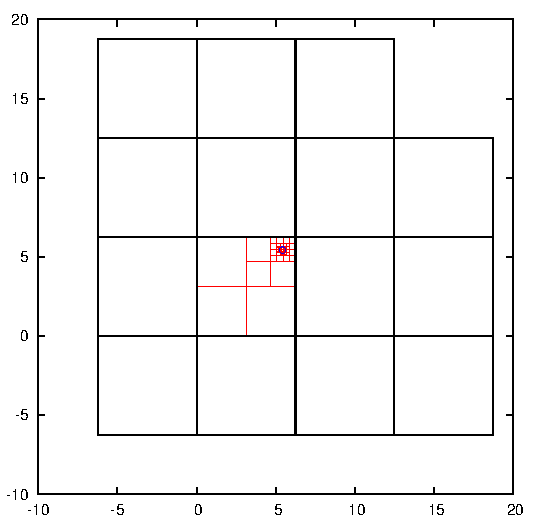
\includegraphics[width=0.45\textwidth]{results/adaptive_refinement_3_old.pdf} }
  \hspace{0pt}
  \subfloat[improved refinement]{\label{fig:adapt_ref_b} 
    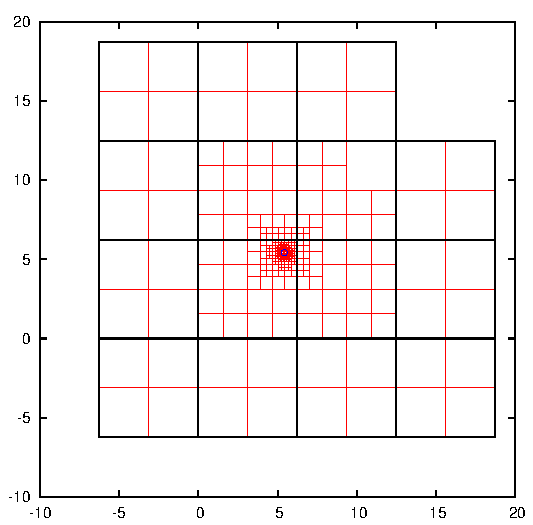
\includegraphics[width=0.45\textwidth]{results/adaptive_refinement_3_new.pdf} }
  \caption[Adaptive refinement comparison]
  {Comparison of the original and improved refinement techniques.
   Black lines denote enriched element edges, red lines denote adaptive refinement (subelement edges) and the well
   edge is blue.
  }
  \label{fig:adapt_refinement}
\end{figure}

We suggested additional criterion for subelements refinement which takes into account a subelement diameter 
and its distance from the well
\begin{equation}
  d_T > C_R|d_{min} - \rho_w|,
\end{equation}
where $d_T$ is the diameter of the subelement and $d_{min}$ is minimal distance between a vertex of 
the subelement and the well edge. $C_R$ is a scaling constant, equal 1.0 by default, through which we can 
control the significance of the criterion.

In this way, the elements in which the well does not lie are also refined as you can see in 
\fig{fig:adapt_ref_b}. The quadrature points are then distributed more 'smoothly' around the well and the
integrals with gradients can be computed more accurately. 

In \fig{fig:adapt_refinement_norm} you can see the $L_2$ norms of the error on the enriched elements which 
were computed also using the corresponding adaptive integration. Notice the scale of the improved version -- 
the error on elements is in small range and is not significantly concentrated anywhere. On the other hand, 
the original version shows out large error that is concentrated on the closest non-refined element to the well.

%\notePE{TODO: add axis, remove legend label, try to sharpen}
\begin{figure}[!htb]
%   \vspace{0pt}
  \centering    
  \subfloat[original refinement]{\label{fig:adapt_ref_norm_a} 
    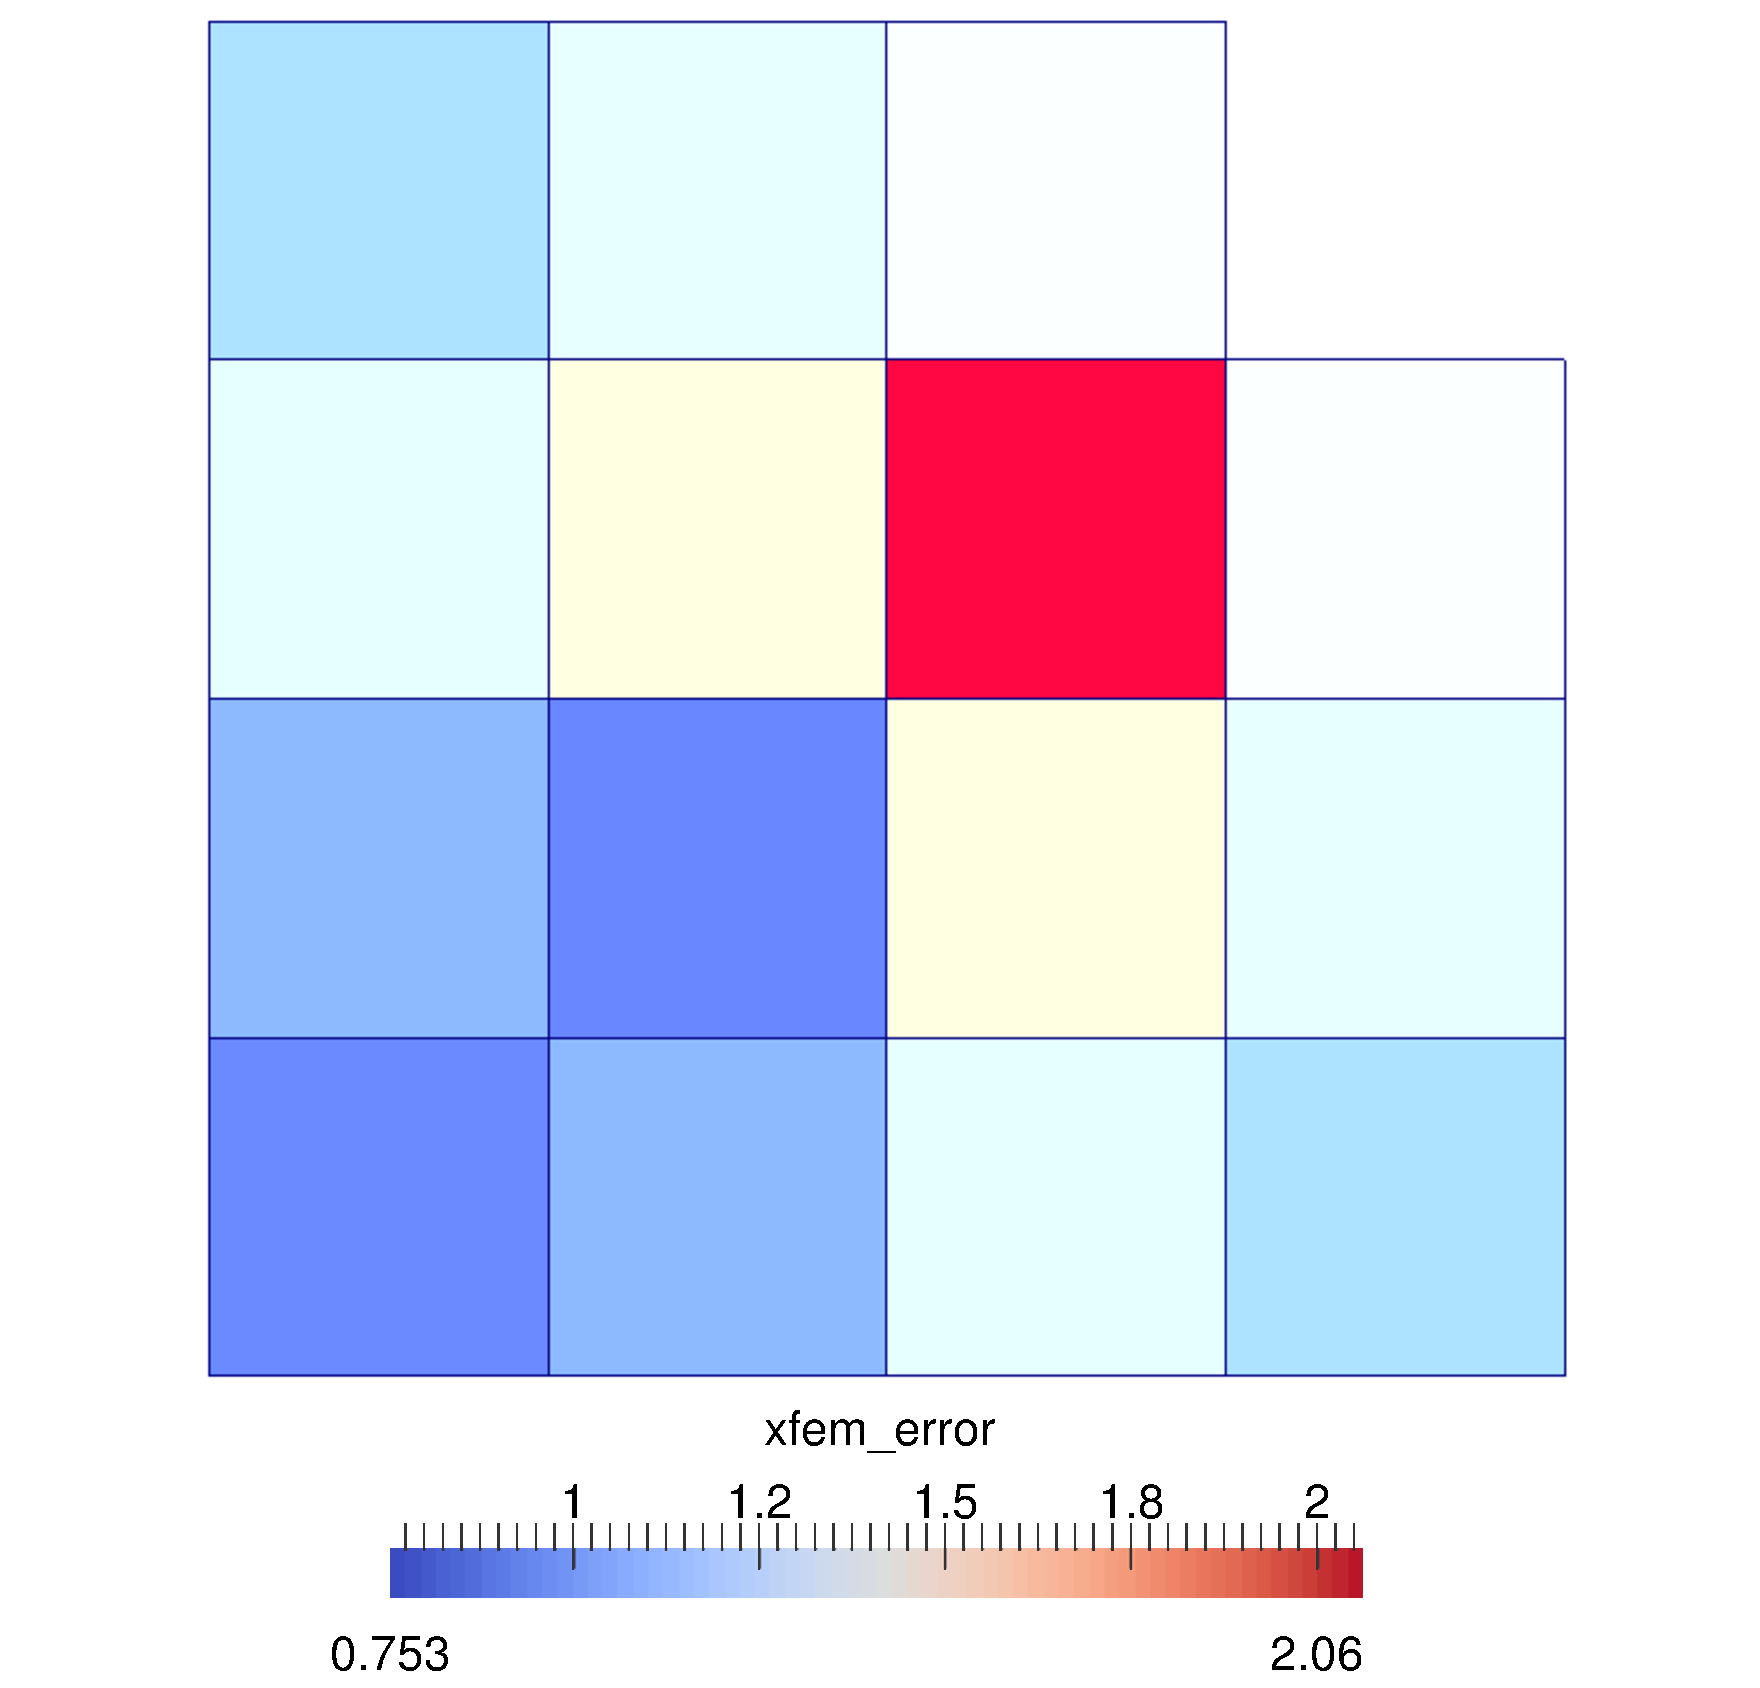
\includegraphics[width=0.45\textwidth]{results/adaptive_refinement_extract_3_old.pdf} }
  \hspace{0pt}
  \subfloat[improved refinement]{\label{fig:adapt_ref_norm_b} 
    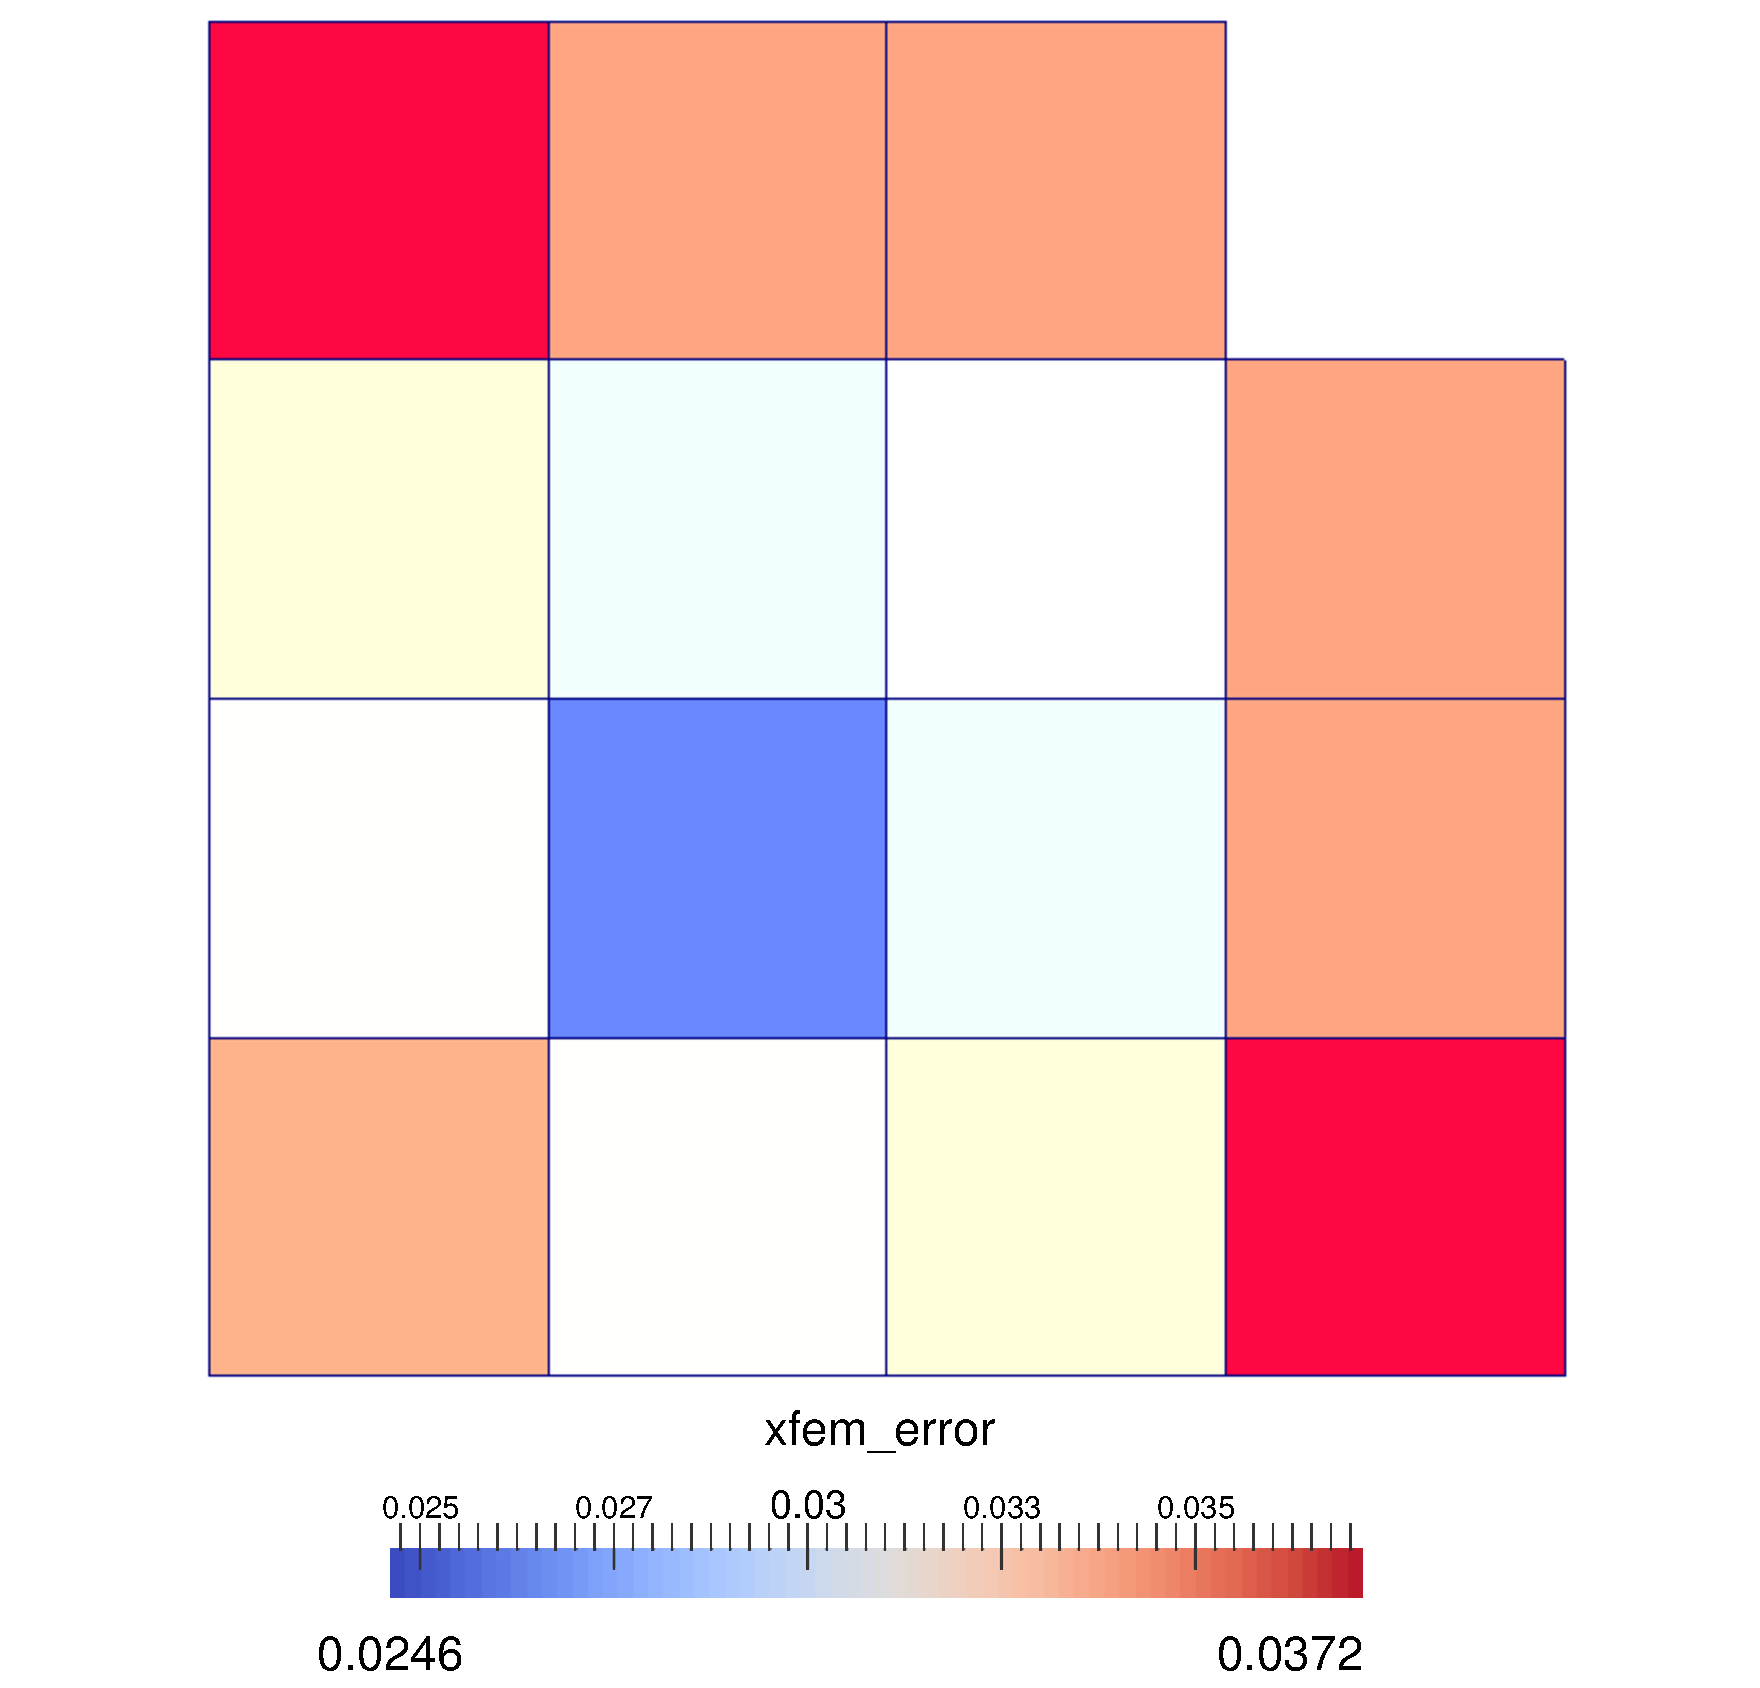
\includegraphics[width=0.45\textwidth]{results/adaptive_refinement_extract_3_new.pdf} }
  \caption[Adaptive refinement comparison]
  {Comparison of element-wise error in $L_2$ norm using different refinement techniques.
  }
  \label{fig:adapt_refinement_norm}
\end{figure}

% \subsection{Circle integration experiment}
% The approximation of the integration domain is also the source of the error. We decided to run 
% an experiment on integrating the characteristic function of the well with our adaptive integration.
% The domain $\Omega$ is a square $4\times4$ out of which a circle of radius 1.0 is cut off. The characteristic 
% function is considered
% \begin{equation}
%   \chi(\bx) = \left\{
%     \begin{array}{l l}
%       0 & \quad \textrm{if } \bx \textrm{ is inside the circle}\\
%       1 & \quad \textrm{otherwise}
%   \end{array} \right.
% \end{equation}
% and the integral 
% \begin{equation}
%   \int_{\Omega}\chi(\bx) \dd\bx = 4^2 - \pi
% \end{equation}
% is equal the area of the square minus the area of the circle.
% 
% In this experiment we investigate the influence of the order of the quadrature rule and the level of
% the refinement on how precisely the well geometry is captured.
% 
% In the graph in \fig{fig:adapt_ref_convergence} we can see that for all the quadratures the convergence rate
% is similar, around 1.5. The gain from using higher order quadratures is not worth, especially in case 
% of the order 4 the error is not much smaller than the error of the quadrature of the order 3. 
% 
% Finally the highest level of refinement is chosen to be 10 and the quadrature order to be 3. The number of
% the quadrature points generated by the process described above in \ref{sec:refinement_element} is then similar 
% both in the original (14793) and improved version (14819).
% 
% \begin{figure}[!htb]
% %   \vspace{0pt}
%   \centering    
%   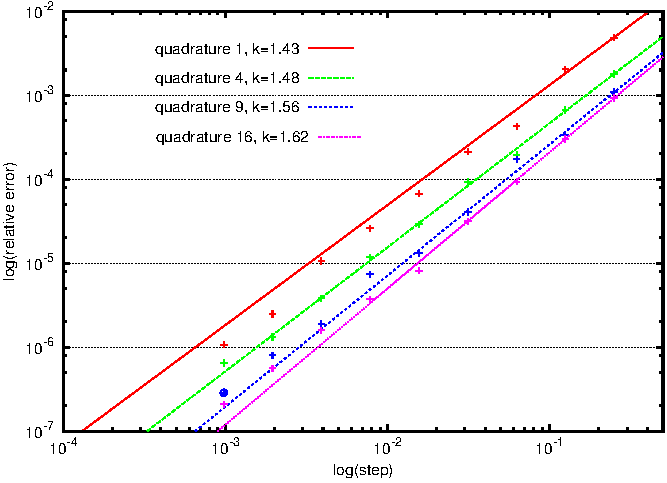
\includegraphics[width=0.7\textwidth]{results/adaptive_integration.pdf}
% %   \subfloat[rozdìlený element s vrtem]{\label{fig:adapt_ref_a} 
% %     \includegraphics[width=70mm]{\figpath adaptive_ref.pdf} }
% %   \hspace{0pt}
% %   \subfloat[detail hranice vrtu]{\label{fig:adapt_ref_b} 
% %     \includegraphics[width=72mm]{\figpath adaptive_ref_detail.pdf} }
%   \caption[Adaptive refinement convergence]{Convergence of adaptive refinement of a circle cutoff.}
%   \label{fig:adapt_ref_convergence}
% \end{figure}

\notePE{
* non-optimal convergence rate with the approach of [gracie] and their integration scheme 3-4\\
* the above can be improved by using higher order quadrature rules (6-6)\\
* problem is that we do not represent the well edge and mainly its surrounding well enough
}

\section{A priori adaptive quadrature}

Let us assume just one well of radius $\rho$ situated at the origin. The worst term to integrate is
\begin{equation}
    \label{eq:term-of-interest}
    f(r)=(\nabla \log r )^2 \approx r^{-2}
\end{equation}
%
independently of the particular variant of the PUM method. Consider a~square $S$ with a~side $h$ and 
let us denote $r_{min}$ and $r_{max}$ the minimum and maximum distance to the origin respectively.
We shall estimate the error of the 2D tensor product Gauss quadrature rule of the order $n$ on the square $S$  
by the error of 1D quadrature of the same order on $(r_{min}, r_{min}+h)$:
\[
  E^n(S) \le h E^n((r_{min}, r_{min}+h)).
\]
This is a conservative estimate, which is natural for elements near the main $x$ and $y$ axis, where the error is maximal.

To guarantee prescribed tolerance $\epsilon$, we want to control the error density
\begin{equation}
    \label{eq:error-density}
     E^n(S) h^{-2} \le h^{-1} E^n((r_{min}, r_{min}+h)) \le \epsilon. 
\end{equation}

Formula for the error of 1D Gauss quadrature of order $n$ ($n$ quadrature points). Quadrature error for $\int_r^{r+h} f$ is 
\[
  E_n = \frac{h^{2n+1} (n!)^4}{(2n+1)((2n)!)^3} f^{(2n)}(\xi_n) 
\]
for some $\xi_n \in (r, r+h)$. 
For the term of interest, i.e. \eqref{eq:term-of-interest}, we have 
\[
  \abs{f^{(2n)}(r)} = (2n+2)! r^{-(2n+2)},
\]
then the convergence criterion following from \eqref{eq:error-density} reads:
\[
  h^{-1}E_n = \alpha_n \left( \frac{h}{r_{min}} \right)^{2n} \frac{1}{r_{min}^2} \le \epsilon, 
  \qquad \alpha_n = (2n+2)\left( \frac{(n!)^2}{(2n)!} \right)^2
\]

Derived criterion holds only on squares, where the integrated function is smooth.
This is not the case for squares intersecting the boundary of the well, $r_{min} \le \rho \le r_{max}$, where we integrate 
discontinuous function $\chi_{S \setminus W} f$. Using substitution, we can map $W$ to unit circle $B$
\[
  \int_{S} \chi_{S \setminus W} \frac{1}{r^2} \d \vc r= \int_{S'} \chi_{S' \setminus B} \frac{1}{r'^2} \d \vc {r'},
\]
where $S'$ is square with side $H=h/\rho$ and $\vc {r'} = \vc{r}/\rho$. Empiricaly determined error of the midpoint rule for later 
integral is
\[
    E(H) = c_e H^{p_e}, \quad \text{with } c_e=0.08,\ p_e=2.5.
\]
This error has to be smaller then $\epsilon h^2$, thus for $h$ we get formula:
\begin{equation} \label{eqn:h_criterion}
   h\le h_b(\epsilon) = \Big(\frac{\epsilon \rho^{p_e}}{c_e}\Big)^{\frac{1}{p_e-2}}. 
\end{equation}

%\noteJB{TODO: modify test of integration on unit disk for the function $1/r^2$.}

Based on the presented analysis above, we propose following rules for adaptive quadrature:
\begin{enumerate}
 \item If $r_{max} < \rho$ the square quadrature is zero.
 \item If $r_{min} < \rho < r_{max}$. For $h \ge h_b(\epsilon)$ subdivide the square, else use lowest order quadrature for 
original function (i.e. $f(r)=0$ for $r\le \rho$).
 \item If $r_{min} > \rho$. For $\frac{h}{r_{min}} > \frac{1}{2}$ subdivide the square, else select order $n$ so that 
 \begin{equation} \label{eqn:alpha_criterion}
    \frac{\alpha_n h^{2n}}{r_{min}^{2n+2}} \le \epsilon,
 \end{equation}
 use at least the same order as necessary for FEM.
\end{enumerate}

\noteJB{TODO:
We should estimate true error numericaly using one more subdivision and compare it to prescribed tolerance, we should be safely 
below, without increasing the number of evaluation comapred to current implementation.
}


\subsection{Adaptive integration experiment}
We now describe the experiment from which we obtained the coefficients in the criterion 
\eqref{eqn:h_criterion}. Let us have a single element, a square $4\times4$, out of which a circle of unit radius 
is cut off -- this represents an element with a well. We now want to investigate integration error
in the vicinity of the circle on the function $f=r^{-2}$, $r$ being the distance from the center of the circle. 

We compute the integral on the selected level of refinement only on the squares intersecting the circle. Then
we refine the squares up to the 12-th level, integrate again and compute the difference. Quadratures rules
$1\times1$, $2\times2$, $3\times3$ and $4\times4$ are used. The results are shown in 
\fig{fig:adapt_integration_conv} also with convergence trend lines equations. The conclusion can be made
that it is more efficient to refine one more level with one-point quadrature than to use higher order 
quadrature on the coarser level. As for the coeffiecient, these can be read from the graph -- for the one point
quadrature $c_e=12.65$ and $p_e=1.27$.

\begin{figure}[!htb]
%   \vspace{0pt}
  \centering    
  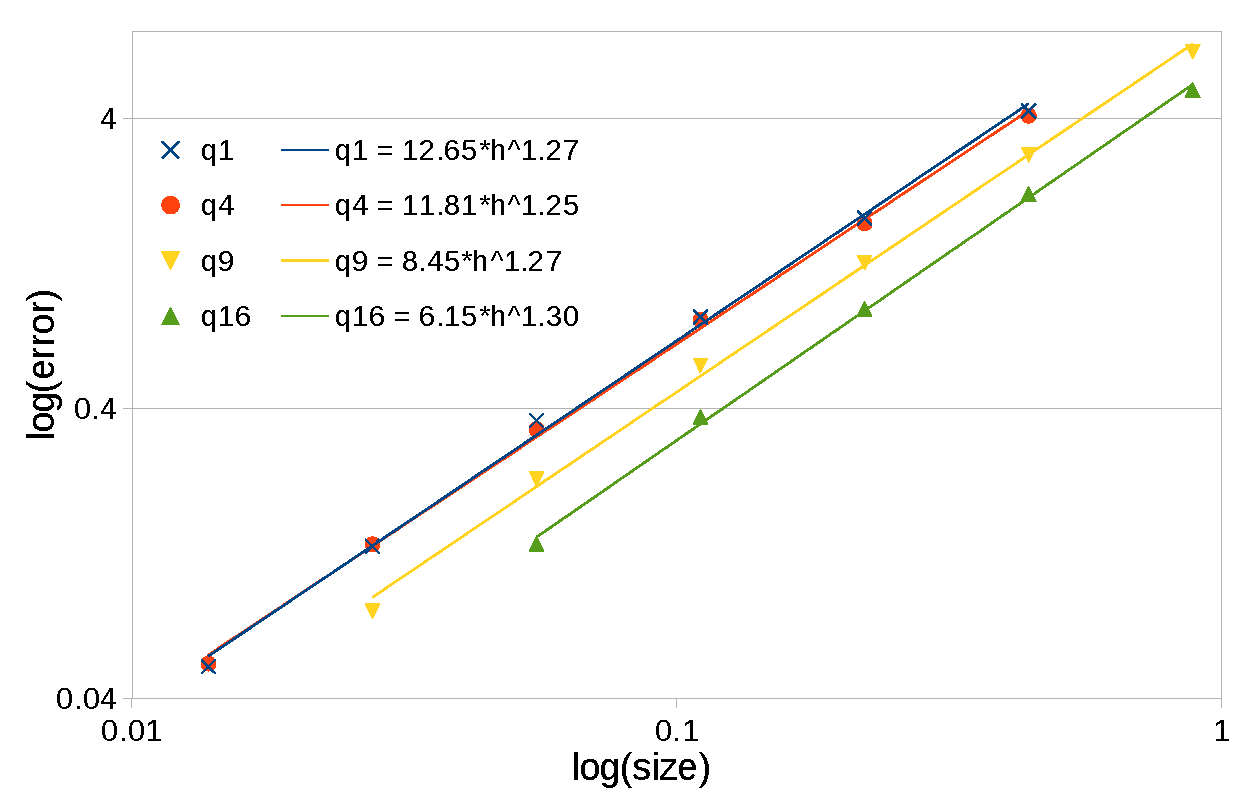
\includegraphics[width=0.9\textwidth]{results/adapt_integration_conv.pdf}
%   \subfloat[rozdìlený element s vrtem]{\label{fig:adapt_ref_a} 
%     \includegraphics[width=70mm]{\figpath adaptive_ref.pdf} }
%   \hspace{0pt}
%   \subfloat[detail hranice vrtu]{\label{fig:adapt_ref_b} 
%     \includegraphics[width=72mm]{\figpath adaptive_ref_detail.pdf} }
  \caption[Adaptive quadrature convergence.]{Convergence graph of adaptive quadrature on function $r^{-2}$.
  \\ \notePE{thicker trend lines}}
  \label{fig:adapt_integration_conv}
\end{figure}

\section{Estimate the enrichment radius}
In this section, we shall study dependance of the solution error on the enrichement radius $R$. First part is devoted to 
theoretical analysis the later part presents numerical results.
Let us consider a general elliptic problem to find $u\in V$ satifying
\[
   a(u, \phi) = \langle f, \phi \rangle, \text{ for } \phi \in V,
\]
where $a$ is bounded elliptic bilinear form: $\norm{a}\le M_a$, $a(v, v) \ge \gamma \norm{v}_V^2$, $\gamma>0$, and $f$ an bounded linear form, $f\in V'$. 
Suppose, that the problem is to be solved on a domain $\Omega \subset \R^2$ with a single hole (well) of radius $\rho$ at the origin. 
Let us assume, that the solution can be splitted to the singular part $u_s(\vc x)= \log |\vc x|$ and the regular part $u_r=u-u_s$.
Let $V^P_h$ be a polynomial finite element subspace of $V$ on a regular mesh of elements with a maximal diameter $h$
and let $V_h$ be a such enriched space that $u_s$ can be approximated exactly on the enrichment zone $Z_R$, i.e.
\[
   \inf_{v\in V_h} \norm{u_s - v}_V = \inf_{v\in V^P_h} \norm{u_s|_{Z'_R} - v}_V, \quad Z'_R = \Omega\setminus Z_R.
\]
Using standard error estimate for eliptic PDE (see e.g. \cite{arnold_lecture_2009}), we get
\begin{equation}
    \label{eq:std_err_estimate}
    \norm{u - u_h}_{V} \le c_a \inf_{v \in V_h} \norm{u - v}_{V} 
    \le c_a \big(\inf_{v \in V^P_h} \norm{u_r - v}_{V} + \inf_{v \in V_h} \norm{u_s - v}_{V} \big).   
\end{equation}
where $c_a=1+\norm{a}/\gamma$.
In the following, we consider $V=H^1(\Omega)$, square grid and $V^P_h$ formed by bilinear finite elements. 
Then \eqref{eq:std_err_estimate} can be further estimated using approximation preperty of $V^P_h$:
\begin{equation}
    \label{eq:particular_estimate}
    \norm{u - u_h}_{V} \le c_a \big(c h \abs{u_r}_{H^2(\Omega)} + \norm{u_s - \Pi u_s}_{H^1(Z'_R)} \big)   
\end{equation}
where $\Pi u_s$ denotes interpolation of $u_s$ in $V^P_h$. Our next aim is to find tight estimate for the second term.
To this end, we calculate $H^1$ error on a single square element $S_{h,r}$ with side $h$ and distance $r$ from origin.
Using parametrization $0<s,t<1$,  we get

\begin{align*}
 (u_s - \Pi u_s)(s,t)&=\log\sqrt{(r+hs)^2+(ht)^2} -\Big[(1-s)(1-t)\log r + (1-s)t\log\sqrt{r^2+h^2}\\
 &\quad+ s(1-t) \log(r+h) + st\log\sqrt{(r+h)^2+h^2} \Big]\\
 &=\frac12 \frac{h^2}{r^2}\big(t^2-t - s^2 +s\big) + O(h^3)
\end{align*}
and 
\begin{equation}
 \nabla(u_s - \Pi u_s)(s,t) = \frac{h}{r^2} \Big( \frac12-s, t-\frac12 \Big) + O(h^2).
\end{equation}
Assuming $h<1$, we can neglect higher order terms. Then by direct integration
\begin{align*}
 \norm{u_s - \Pi u_s}^2_{L^2(S_{h,r})} \approx \frac14 \frac{h^6}{r^4}\int_0^1\int_0^1 (t^2-t-s^2+s)^2\,\d s\, \d t = \frac{1}{360}\frac{h^6}{r^4} 
\end{align*}
and
\begin{align*}
 \norm{\nabla(u_s - \Pi u_s)}^2_{L^2(S_{h,r})} \approx \frac{2h^4}{r^4} \int_0^1 \Big(t-\frac12\Big)^2 \d t = \frac{1}{6}\frac{h^4}{r^4}.
\end{align*}
Thus for the density of squared error we obtain 
\[
    \frac{1}{\abs{S_{h,r}}} \norm{u_s - \Pi u_s}^2_{H^1(S_{h,r})} \approx \frac{h^2}{6r^4}
\]
and we can estimate
\[
  \norm{u_s - \Pi u_s}_{H^1(Z'_R)} \le \left[\int_0^{2\pi} \int_R^\infty \frac{h^2} {6r^4} r \,\d r\, \d \phi\right]^{1/2} = \sqrt\frac{\pi}{6}\frac{h}{R}.
\]
Recalling the estimate \eqref{eq:particular_estimate}, we can conclude that optimal choice of the enrichment radius is $1/R\approx \abs{u_r}_H^2(\Omega)$, 
which balance error in the regular and the singular part. \noteJB{Possible remarks: General form of the error; automatic choice via aposteriori error estimates
$R \approx h/\norm{u-u_h}_{H^1}$.}



We confirm the validity of the estimate \eqref{eqn:log_h1_estimate} in 2D case by a numerical test.
The ratio 
\begin{equation} \label{eqn:log_h1_estimate_ratio}
\frac{h^{3/2} r^{-2} 12^{-1/2}}{\|\log \vc x - u_h\|^2_{H^1(T)}}
\end{equation}
is computed on every element $T$ of the mesh using a $5\times5$ Gaussian quadrature, with $h$ being the 
element diameter and $r$ being the distance between the element center and the origin. The results on five
refined meshes are gathered in the table \ref{tab:log_h1_estimate}. 
%
\begin{table}
\begin{center}
\begin{tabular}{crr}
\toprule
% \multicolumn{2}{c}{Item} \\
% \cmidrule(r){1-2}
$h$    & min & max \\
\midrule
$\rfrac{14}{8}$   & 0.97 & 7.1  \\% & 1.38 & 10.0  \\ %& 0.7 & 5.3   \\
$\rfrac{14}{16}$  & 0.99 & 16.4  \\% & 1.40 & 23.1  \\ %& 1.0 & 17.4  \\
$\rfrac{14}{32}$  & 1.00 & 34.4  \\% & 1.41 & 48.7  \\ %& 1.5 & 51.8  \\
$\rfrac{14}{64}$  & 1.00 & 70.3  \\% & 1.41 & 99.5  \\ %& 2.1 & 150   \\
$\rfrac{14}{128}$ & (0.756) 1.00 & 142.0   \\% & 1.41 & 201   \\ %& 3.0 & 427   \\
\bottomrule
\end{tabular}
\caption{Numerical validation of the estimate \eqref{eqn:log_h1_estimate} in 2D case. The minimal and maximal 
values of \eqref{eqn:log_h1_estimate_ratio} are collected in the table for different refinements.
\notePE{DONE: Seems that there is still a coeffient close to $\sqrt{2}$.}}
\label{tab:log_h1_estimate}
\end{center}
\end{table}
%
We can see from the 'min' column of the table \ref{tab:log_h1_estimate} that the ratio is very close to 1.0 
which means we have a good upper estimate. 
The value in brackets at the finest refinement pertains to several elements near the well where the used 
quadrature is too coarse. However the ratio is greater than or equal 1.0 elsewhere.

Further we can see the error in $H^1$ norm over the elements in the \fig{fig:log_estimate_a}. We can 
compare it with the ratio in the \fig{fig:log_estimate_b} and see that the ratio iis closest to 1.0 
(our estimate is best) where the error is largest 
(in $x$ and $y$ directions) and otherwise in diagonal directions. We can also notice that the logarithm is 
better approximated by the linear functions in the diagonal directions than in the axes directions.

\begin{figure}[!htb]
%   \vspace{0pt}
  \centering    
  \subfloat[$\|\log \vc x - u_h\|^2_{H^1(T)}$ in log scale]{\label{fig:log_estimate_a} 
    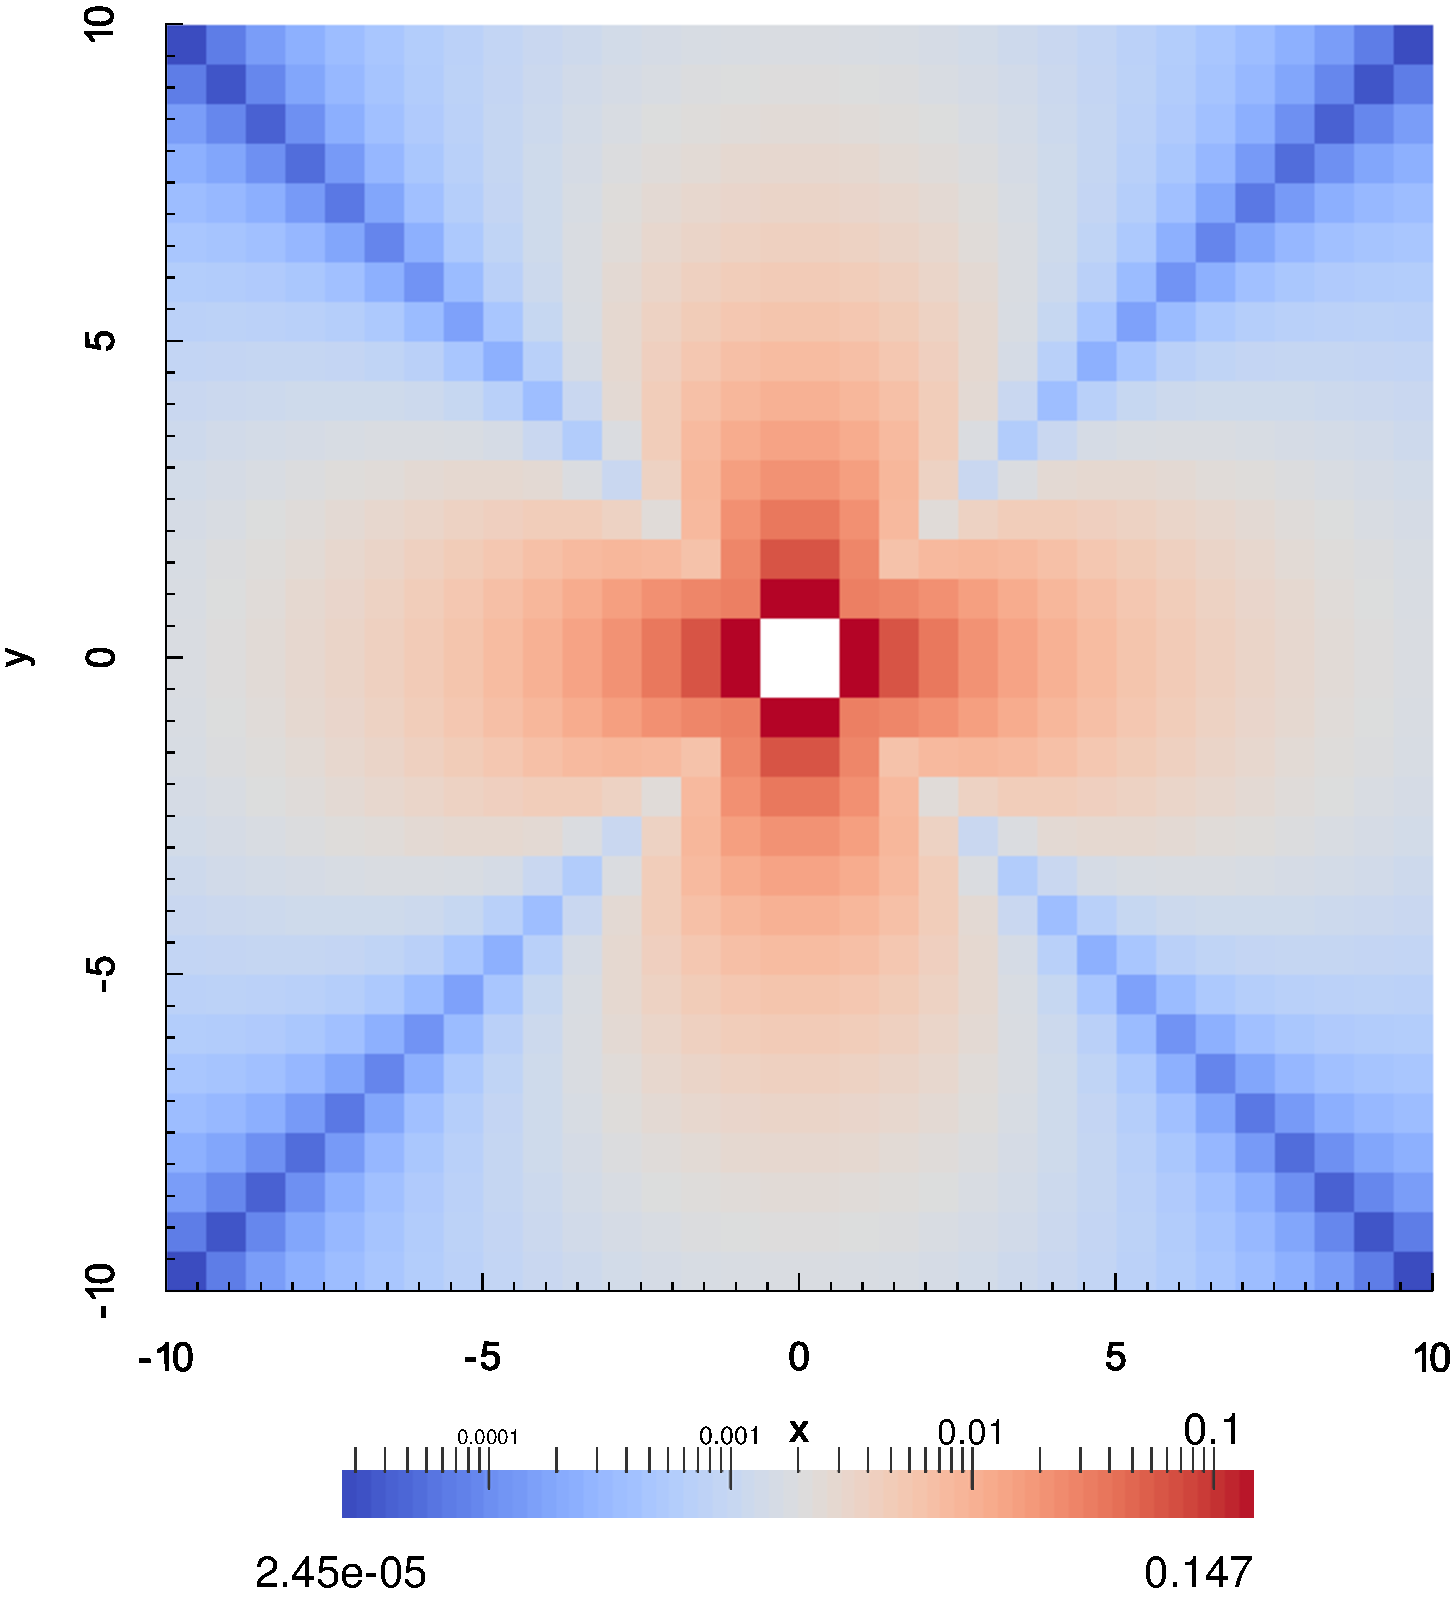
\includegraphics[width=0.47\textwidth]{results/log_estimate_h1.pdf} }
  \hspace{0pt}
  \subfloat[the ratio \eqref{eqn:log_h1_estimate_ratio}]{\label{fig:log_estimate_b} 
    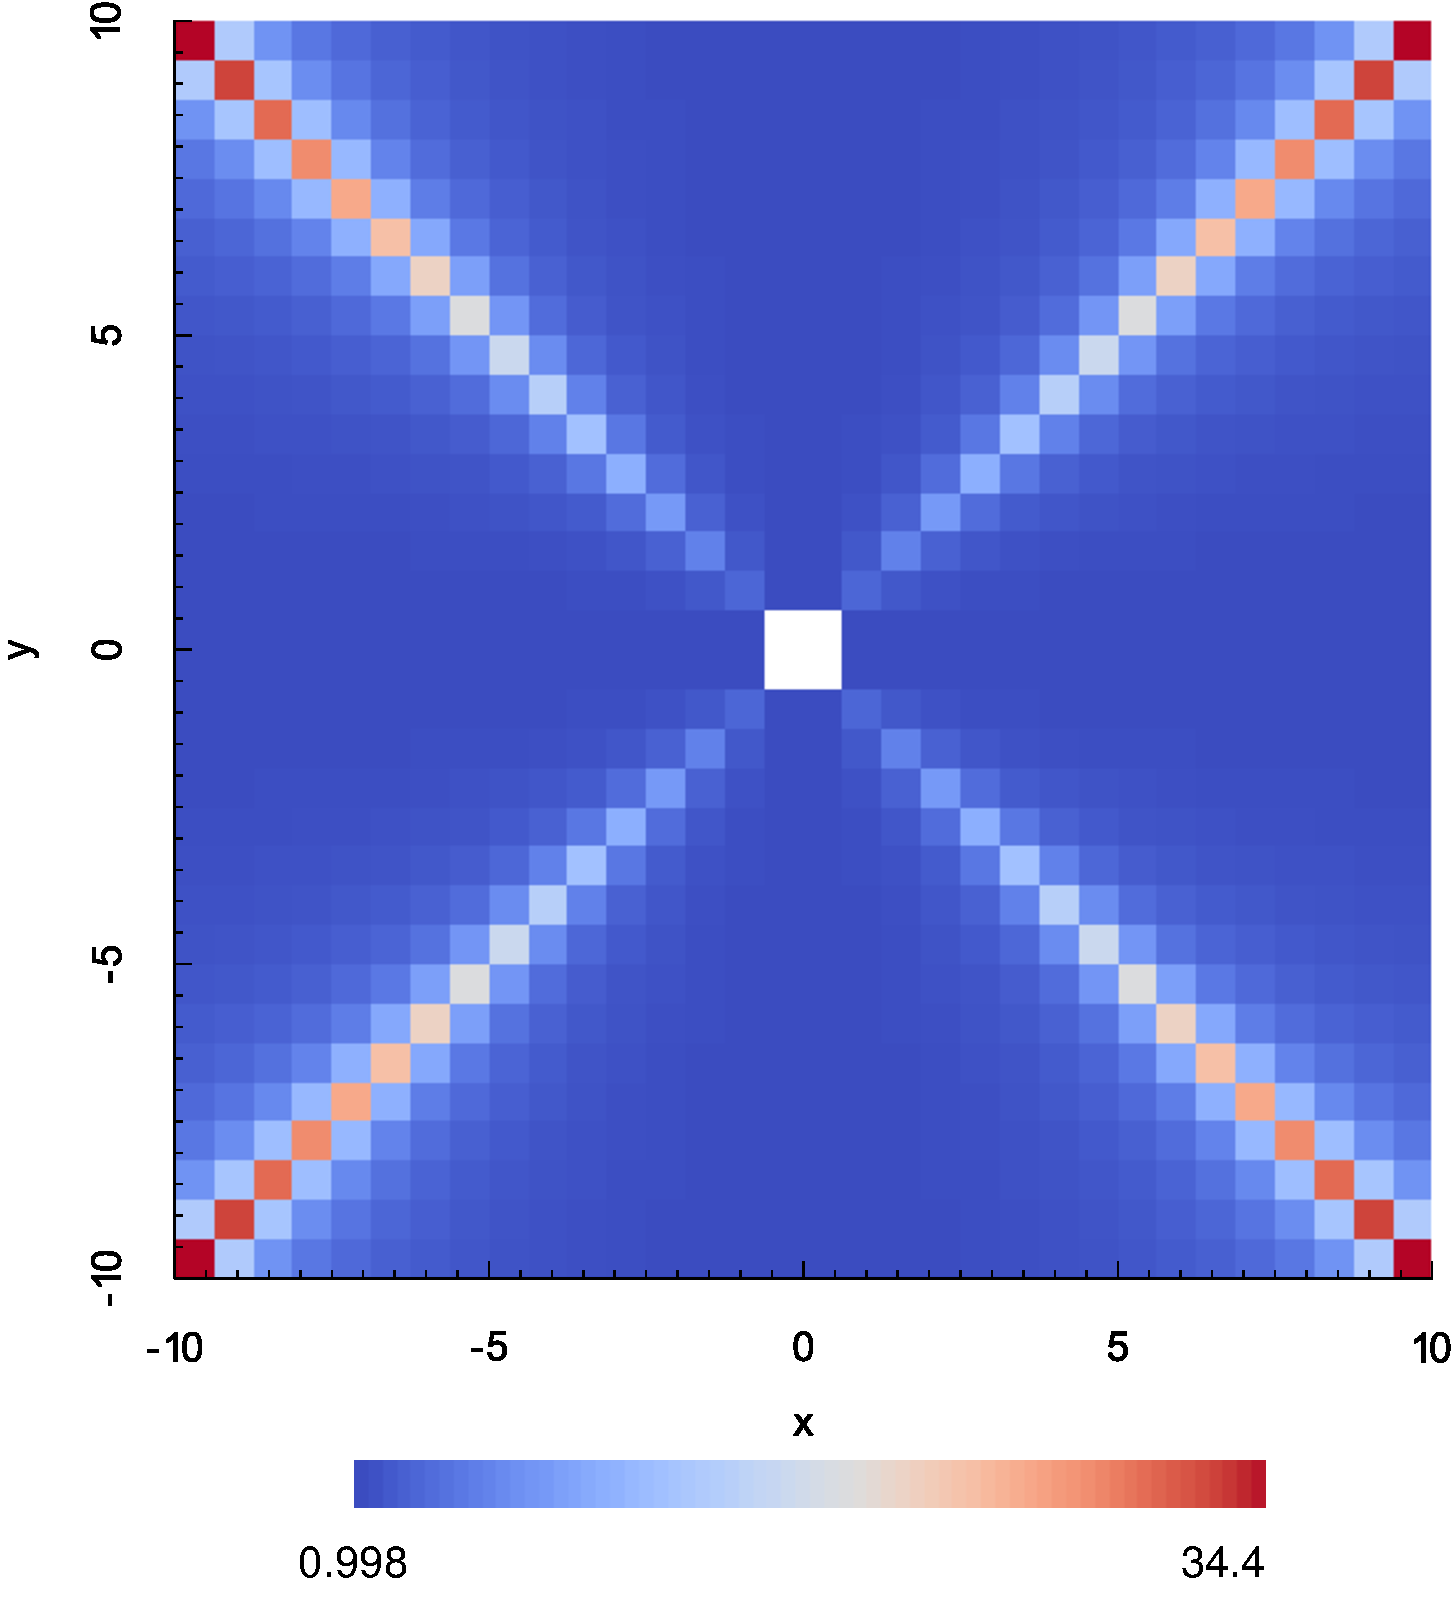
\includegraphics[width=0.47\textwidth]{results/log_estimate_ratio.pdf} }
  \caption[Log error estimate.]
  {\notePE{Exchange figures with correct scales -- after running corrected test.}
  Results of the numerical validation of the estimate \eqref{eqn:log_h1_estimate}. The elements are left out 
  in the center where the $\log$ singularity is situated and where the function is cut off.
  }
  \label{fig:log_estimate}
\end{figure}



We demonstrate the behaviour of the model depending on the enrichment radius choice on our test case with 
source term present. \notePE{Define the two test case - with and without source.}
The convergence graph in \fig{fig:radius_conv_1} shows how the error depends on the element size for different 
enrichment radius. As a reference in the graph, we added the error of classical FEM applied on the same problem 
but with well omitted -- the convergence rate is optimal 2.0. We see that the convergence rate for all the 
chosen enrichment radii is very close to the optimum. It is degraded for smaller element size while we are
approaching the accuracy limits of the integration.

We also see in \fig{fig:radius_conv_1} that the error is not decreasing significantly for larger enrichment 
radii. This trend is more obvious from the graph in \fig{fig:radius_conv_2} which shows the dependance of the
error on the enrichment radius for different element sizes.

\begin{figure}[!htb]
%   \vspace{0pt}
  \centering    
  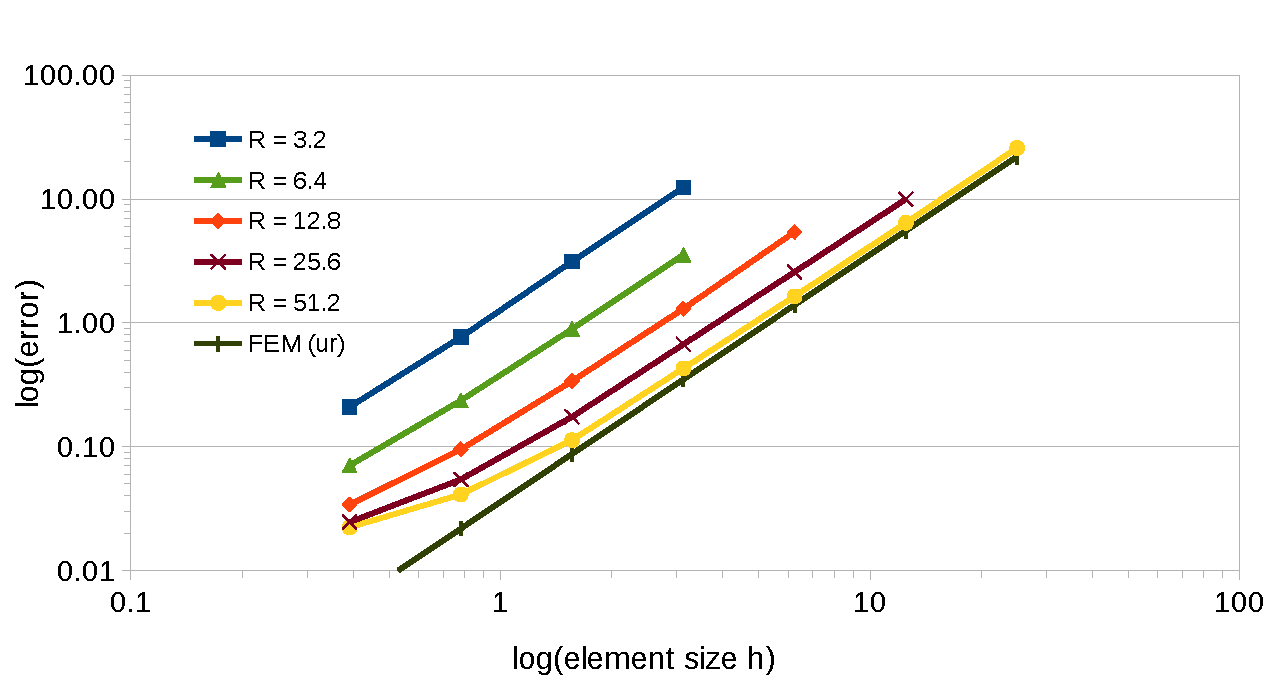
\includegraphics[width=0.9\textwidth]{results/radius_conv_1.pdf}
%   \subfloat[rozdìlený element s vrtem]{\label{fig:adapt_ref_a} 
%     \includegraphics[width=70mm]{\figpath adaptive_ref.pdf} }
%   \hspace{0pt}
%   \subfloat[detail hranice vrtu]{\label{fig:adapt_ref_b} 
%     \includegraphics[width=72mm]{\figpath adaptive_ref_detail.pdf} }
  \caption[Enrichment radius choice.]{Convergence graph for different enrichment radii. The 'FEM sin(x)'
  data comes from the problem without well solved by classical FEM and with optimal convergence rate 2.0.}
  \label{fig:radius_conv_1}
\end{figure}
\begin{figure}[!htb]
%   \vspace{0pt}
  \centering    
  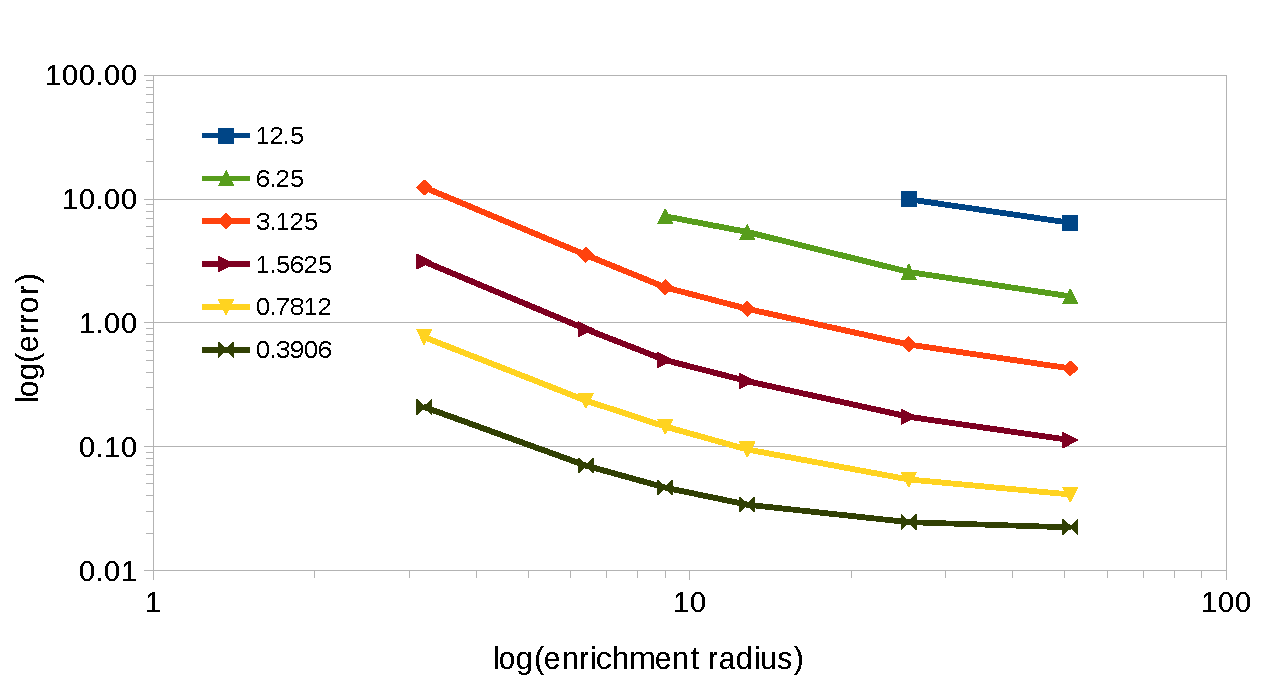
\includegraphics[width=0.9\textwidth]{results/radius_conv_2.pdf}
%   \subfloat[rozdìlený element s vrtem]{\label{fig:adapt_ref_a} 
%     \includegraphics[width=70mm]{\figpath adaptive_ref.pdf} }
%   \hspace{0pt}
%   \subfloat[detail hranice vrtu]{\label{fig:adapt_ref_b} 
%     \includegraphics[width=72mm]{\figpath adaptive_ref_detail.pdf} }
  \caption[Enrichment radius choice.]{Dependence of the error on the enrichment radius for different
  element sizes.}
  \label{fig:radius_conv_2}
\end{figure}

\section{Condition number}
Condition number for matrices resulting from conforming FEM applied to Laplace equation is $O(h^{-2})$, so the iteration count 
for CG without preconditioning is $O(h^{-1})=O(\sqrt(n))$, where $n=1/h^2$ is number of DOFs. With local preconditioning (Jacobi, 
SOR, ILU) one can usually achieve number of iteration $O(h^{-0.5})$, c.f. \cite{ern_evaluation_2006}.


\section{Results}
\label{sec:results}
In this section we present the main results. We solve \probref{def:test_case_1} and \probref{def:test_case_2} 
defined in section \ref{sec:test_cases} with the methods described in \ref{sec:pum_methods} and compare them.

Let us start with the \probref{def:test_case_1} and look at the convergence graph in \fig{fig:convergence}.
At first we solve the problem by standard FEM with adaptive mesh refinement where 30\% of the elements
with the highest error estimate are refined (the element size is then taken at the smallest elements in the 
vicinity of the well). We see that the convergence is slow until the size of elements reaches the scale of the
well. Therefore we divided the graph in two parts with convergence rates 0.56 and 1.27.



\begin{figure}[!htb]
%   \vspace{0pt}
  \centering    
  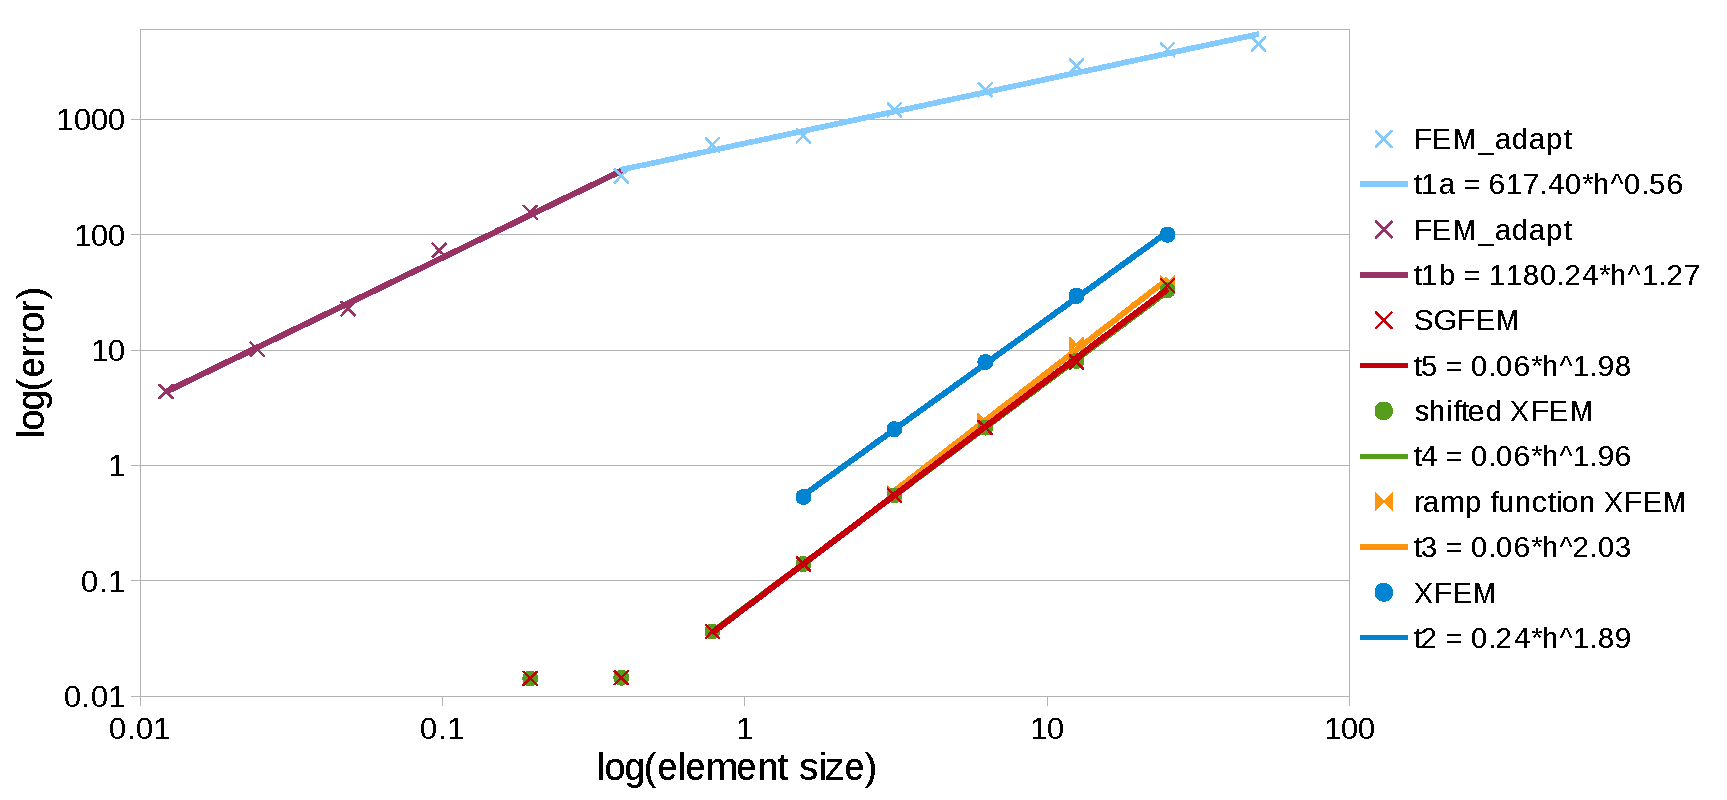
\includegraphics[width=\textwidth]{results/convergence.pdf}
  \caption[Convergence graph \probref{def:test_case_1}]{Convergence graph of different methods on 
  \probref{def:test_case_1}. }
  \label{fig:convergence}
\end{figure}
\begin{figure}[!htb]
%   \vspace{0pt}
  \centering    
  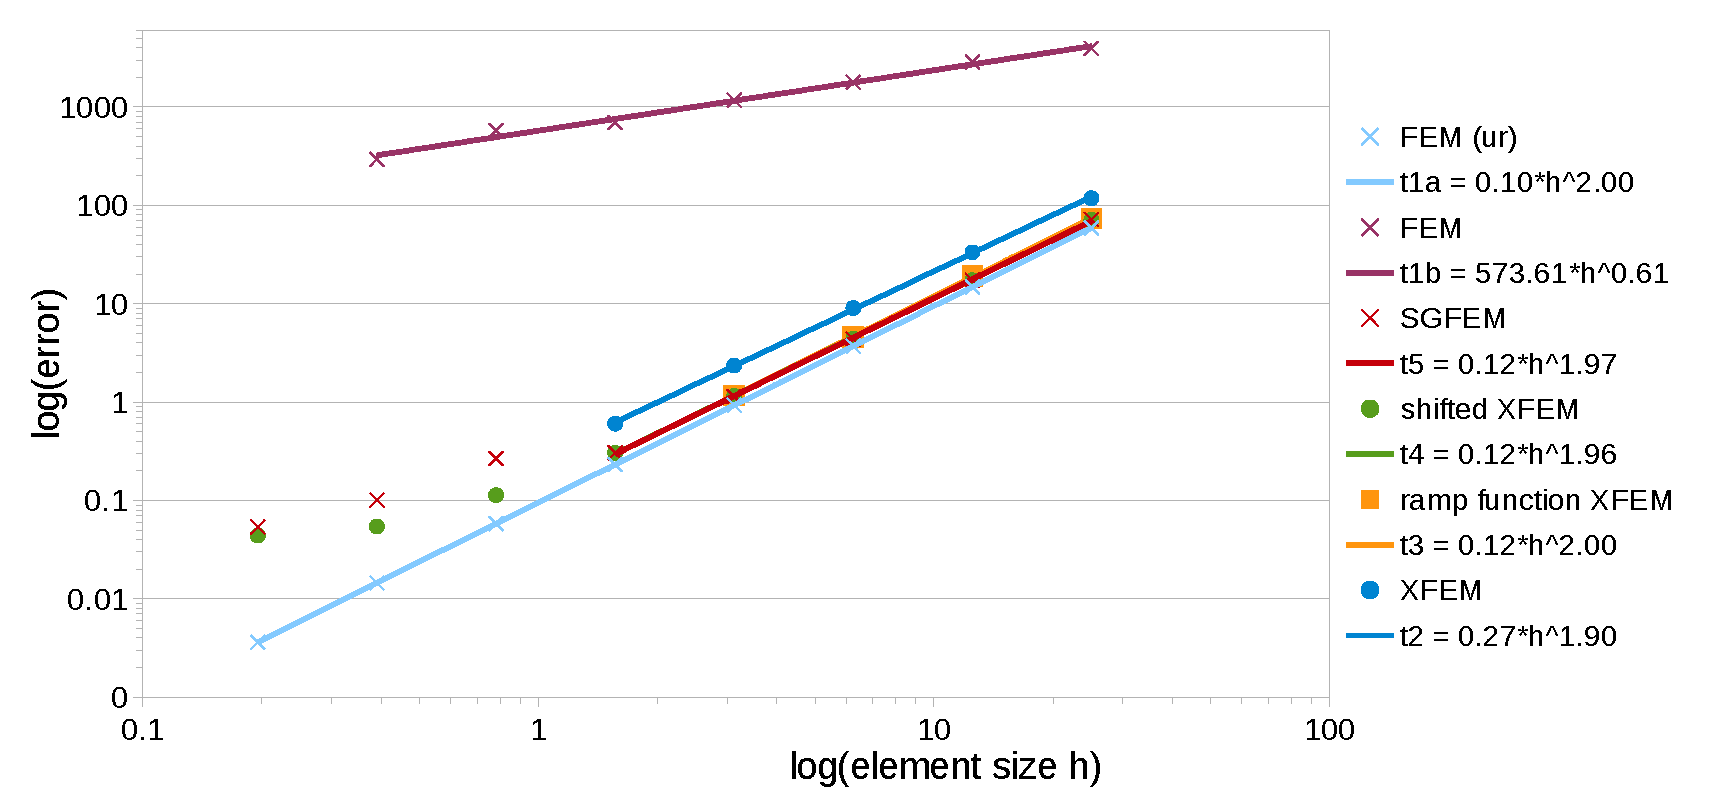
\includegraphics[width=\textwidth]{results/convergence_sin.pdf}
  \caption[Convergence graph \probref{def:test_case_2}]{Convergence graph of different methods on 
  \probref{def:test_case_2}. The 'FEM sin(x)'
  data comes from the problem without well solved by classical FEM and with optimal convergence rate 2.0.}
  \label{fig:convergence_sin}
\end{figure}


\section{Summary}
\label{sec:summary}

\section{Acknowledgement}
This work was made under the sincere guidance and support of Mgr. Jan B{\v r}ezina, Ph.D.

This work was supported by the Ministry of Education of the Czech Republic within the SGS project 
no. 21066/115 on the Technical University of Liberec.

%% The Appendices part is started with the command \appendix;
%% appendix sections are then done as normal sections
%% \appendix

%% \section{}
%% \label{}

%% If you have bibdatabase file and want bibtex to generate the
%% bibitems, please use
%%
%%  \bibliographystyle{elsarticle-harv} 
%%  \bibliography{<your bibdatabase>}

%% else use the following coding to input the bibitems directly in the
%% TeX file.

% \begin{thebibliography}{00}
% 
% %% \bibitem[Author(year)]{label}
% %% Text of bibliographic item
% 
% \bibitem[ ()]{}
% 
% \end{thebibliography}
 %\nocite{dip}
 %\bibliographystyle{elsarticle-harv} 
 %\bibliographystyle{elsarticle-num-names} 
 \bibliographystyle{elsarticle-num} 
 \bibliography{../citace.bib}
\end{document}

\endinput
%%
%% End of file `elsarticle-template-harv.tex'.

